\documentclass[12pt,openany]{book}
\usepackage{verbatim}
\usepackage{libertinus}
\usepackage{hyperref}
\usepackage[margin=1.0in]{geometry}
\usepackage{titlesec}
\usepackage{chronology}
\usepackage{quotchap}
\usepackage[style=numeric,backend=biber,url=true]{biblatex}
\usepackage{tikz}
\usepackage{luacode}
\addbibresource{refs.bib}

\fontfamily{libertinus}
\titleformat{\chapter}[frame]
  {\normalfont\huge\bfseries}{\thechapter}{0.5em}{\Huge\centering}
\titlespacing{\chapter}{0pt}{0pt}{40pt}

\title{A Brief History of Compilers}
\author{Asher Mancinelli}
\date{}

\begin{document}

\directlua{
  timeline = require("timeline")
}

\maketitle
\tableofcontents

\newcommand{\tex}{\TeX\hspace{0.3em}}
\newcommand{\metafont}{\texttt{METAFONT}}

\newcommand{\chapterstar}[1] {
\chapter*{#1}
\addcontentsline{toc}{chapter}{#1}
}

\newcommand{\longcite}[1]{\citetitle{#1}, \textcite{#1}}


\chapterstar{Preface}

The history of compilers is rich and deeply connected to the broader history of computing,
however, I believe that no comprehensive work has tied together the threads of this history
with a specific focus on compilers.
There are wonderful tellings of the very first compilers on Konrad Zuse's Z4 computer at the ETH Zurich
and Grace Hopper's pioneering work on the A-series compilers for the UNIVAC I,
and John Backus' work on the first commercial compiler for \FTN{} at IBM,
but these are often isolated stories.
When they are woven together, they are often not connected to the
\textit{next} developments in compiler technology at Bell Labs:
Aho and Ullman's \textit{Principles of Compiler Design}, the development of Lex and Yacc,
the C programming language, Bjarne Stroustrup's first C++ compiler \texttt{cfront}
(inspired by Alan Kay's vision of object-oriented programming).
The subsequent decades of open-source compiler development, advances in optimization techniques,
and the explosion of new programming languages and compilation paradigms
(e.g. just-in-timem compilation) are then followed by the
rise and necessity of hardware-software codesign and domain-specific languages
seen most evidently in projects based on MLIR and LLVM.
The threads between these points in history offer a deeper understanding of
each individual piece and context that motivates modern compiler development.
\C{snipped text.}{
There have been several monumentous works on the history of computing and a few on
the history of programming languages, but in the two and a half decades since the turn
of the century there have been ample developments in compiler technology that
no comprehensive work has covered thus far.
This book aims to fill that gap to a small degree; it is not exhaustive, but
contextualizes many of the most important recent developments in the larger
narrative of compiler history.
}

% The introduction chapter contains a brief version of the entire book; the reader is encouraged to read it first.
This work intends to weave these threads together.
My hope is that each chapter stands on its own, but that reading them in order will give a more complete picture.
The reader ought to be able to read a particular chapter that suits their needs at the time.
This book does not assume the reader is deeply familiar with compiler engineering or computer science.
The book is structured as a chronological narrative of the history of compilers,
intending to keep the focus on compiler technologies and the people behind them
without focusing on any particular company or product.

\chapter{Introduction}

While the modern programmer may consider the term \emph{compiler} to be a specific one, it is specific only in the
sense that users of the word tend to mean the same thing when they say it.
The details of what a compiler does are often obscure to even professional software engineers.
This is especially evident when they feel the need to use a term like \emph{transpiler} to distinguish between a
"true" compiler and one that emits code another programming language.
Of course, to someone more familiar with the workings of compilers, this distinction is not so useful.
Brian Kernighan described compilers in this seemingly general way\cite{new_history_of_modern_computing}:

\begin{quotation}
\textit{
A compiler is a program that translates something written in one language into something semantically equivalent in another language.
For example, compilers for high-level languages like C and Fortran might translate into assembly language for a particular kind of computer; some compilers translate from other languages such as Ratfor into Fortran.
}
\end{quotation}

However, this is not sufficiently general.
Two key counter examples are \tex and \metafont, which are compilers that
transform text into PDF documents and renderable fonts.
Transforming text into an executable program is not the same process as
transforming text into a document or font, yet both are considered compilation.

When students are first introduced to compilers, the first sort of program they are contrasted with is interpreters.
This distinction is not necessarily meaningful either.
The conventional notion of an interpreter is a program that performs the actions
specified by the source code as chunks of the code are consumed;
perhaps this was the case with early \texttt{BASIC} interpreters
and it may be a useful mental model when introducing interpreters to new programmers,
but one is hard-pressed to find a modern interpreter that does not perform some sort of compilation step.
The most popular interpreters for today's most popular interpreted languages,
Python and Javascript, both use relatively sophisticated compilation techniques.
There are even many Python \textit{libraries} that perform
just-in-time (JIT) compilation, targetting CPUs, GPUs, and other specialized hardware
\cite{jax-compiler}\cite{lam_numba}\cite{numba_cuda}\cite{triton_tillet}.

\vspace{0.5em}

To capture the full spectrum of compiler technologies,
the definition we will use in this book is intentionally broad:
\begin{quotation}
\textit{
    A compiler analyzes, transforms, and produces code, based on source code.
}
\end{quotation}

In the case of \tex and \metafont, the source code
may not entail a \textit{program} in the conventional sense;
\tex source code describes a document rather than a sequence of
instructions to be performed.
The code being produced by the compiler may be the encoded PDF format, for instance.
So too are interpreters which produce code in some form during the interpretation process.
The CPython interpreter produces bytecode before executing the program,
meaning it is a compiler by our definition.
Perhaps CPython it is a compiler the consumes Python code and produces CPython bytecode,
which also happens to ship a CPython bytecode virtual machine which typically
executes the bytecode as soon as it is produced.

The point of this section is not pedantry, but to establish a broad definition of
compiler technology before embarking on the details of its development.

We will primarily focus on compilers that actually ran on a machine at one point.
We largely exclude theoretical works like Ada Lovelace's notes on claculating Bournoulli numbers
and the development of automata, for instance.
Each step in the development of compiler technology builds on the previous steps,
and while they are important, our focus is on compiler programs and not the
primarily theoretical or pen-and-paper works that preceded them.

\chapter{Dawn, 1940-1960}
\section{Where Does it Start?}
There is significant debate about who created the first compiler,in no small
part due to ambiguous nomenclature.The term \textit{software} came into use
sometime between 1959 and 1962,as \citeauthor{the-first-computers-2002} note:
\begin{quotation}
  [Expressions] such as "hardware", "software", "machine language",
  "compiler", "architecture" and the like... were unknown in 1950.
  They only arrived a decade later, but the underlying concepts were
  quite familiar to us.
  \cite{the-first-computers-2002}
\end{quotation}

This Honeywell advertisement \textit{A Few Quick Facts on Software} sought to
clarify these terms as well:

\begin{quotation}
  Software is a new and important addition to the jargon of computer
  users and builders.It refers to the automatic programming aids that
  simplify the task of telling the computer 'hardware' how to do its
  job\dots
  % Generally there are three basic categories of software:
  % 1) Assembly Systems, 2) Compiler Systems, and 3) Operating Systems.
  \cite[ch.5]{new-history-of-modern-computing}
\end{quotation}

At this time, hardware was the only piece that mattered to customers.Software
was an afterthought, if a thought at all.The instruction set of the machine was
important, because that was the user's interface to the machine.It should come
as no surprise, then, that the origins of our modern understanding of the term
\textit{compiler} are similarly murky, especially considering the fact that
\textit{compiler} already carried meaning in English, and was repurposed for
computing.John Backus even pointed out how the ambiguity around the term
\textit{compiler}makes computing history ca 1950s especially difficult to
untangle:
\begin{quotation}
  There is an obstacle to understanding, now, developments in
  programming in the early 1950s. There was a rapid change in the
  meaning of some important terms during the 1950s. We tend to assume
  that the modern meaning of a word is the same one it had in an early
  paper, but this is sometimes not the case. Let me illustrate this
  point with examples concerning the word "compiler."
  \cite{Backus_1980_Programming_in_America_in_1950s}
\end{quotation}
\bigskip
Once could argue that any of these efforts constituted the first compiler:
\begin{itemize}
  \item Konrad Zuse's run-programs for the Z4 at the ETH Zurich in 1950
  \item Grace Hopper's A-0 and A-1 compilers for the UNIVAC I at
    Remington Rand in 1951
  \item Laning and Zierler's algebraic compiler for the Whirlwind at MIT in 1950
  \item John Backus's \FTNI{} compiler at IBM
\end{itemize}

I attempt to discuss these in order, however their efforts overlap
significantly in time.I try to tell their stories as a whole, though each story
contains references to the others;if you find yourself confused by names
introduced out of context, please finish the chapter or search for the content
within this chapter before giving up.
\section{Development of the Z4}
Konrad Zuse, a German civil engineer, began work on the Z4 during World War
II.Funded partially by his family and partially by the Nazi government, his
prior works demonstrated significant creativity and ingenuity, and they were
leveraged to build precursors to modern cruise missiles and guided bombs.Most of
Zuse's machines prior to the Z4 were destroyed during the war. \todo{Zuse's Z4
  was a strange machine with bespoke memory and instruction set.This
  affected how
the compilers for it were designed.} In a turn of events Konrad Zuse was made
aware of Aiken's Mark I through his daughter:
\begin{quotation}
  Konrad Zuse told me an amusing anecdote about how he first
  encountered the work of Aiken. The occasion of our conversation was
  a luncheon in Zuse's honor, hosted by Ralph Gomory at the Watson
  Research Laboratory of IBM before a lecture given by Zuse to the
  staff of the lab. When Zuse learned that I was gathering materials
  for a book on Aiken, he told me that he had come across Aiken and
  Mark I in an indirect manner, through the daughter of his
  bookkeeper. She was working for the German Secret
  Service (Geheimdienst) and knew through her father of Zuse's work on
  a large scale calculator. According to Zuse,the young woman never
  learned any details about his machine, which was shrouded in
  war-time secrecy. But she knew enough about Zuse's machine to
  recognize that the material filed in a certain drawer related to
  advice that seemed somewhat like Zuse's. She reported this event
  to her father, giving the file number of the drawer, and the father
  at once informed Zuse of her discovery. Zuse, of course, could not
  go to the Secret Service and ask for the document since that would
  give away the illegal source of his information. Zuse was well
  connected, however, and was able to send two of his assistants to
  the Secret Service, armed with an official demand for information
  from the Air Ministry,requesting any information that might be in
  the files concerning a device or machine in any way similar
  toZuse's.Zuse's assistants were at first informed that no such
  material existed in the files, but they persisted and eventually got
  to the right drawer. There they found a newspaper clipping (most
  likely from a Swiss newspaper), containing a picture of Mark I and a
  brief description about Aiken and the new machine. But there was not
  enough technical information to enable Zuse to learn the machine's
  architecture.
  \cite{howard_aiken_and_the_dawn_of_the_computer_age_2000}
\end{quotation}
\section{The ETH's Acquisition of the Z4}
There were several early efforts to create programs that produced punch
cards which contained machine code instructions, which could then be fed back
into the machine as input punchcards.The programs produced by these early
compilers were called \textit{run-programs}, and the process of using them was
called \textit{automatic programming}, a term later coined by Grace Hopper.The
first of these programs was run on a machine called the Z4, designed by Konrad
Zuse in Germany.Professor Eduard Stiefel, shortly after establishing the
Institute of Applied Mathematics to study numerical analysis at the Swiss
Federal Institute of Technology (ETH) in Zurich,began searching for a computer
for the institute.He learned of the computing advancements in the United
States, Great Britain, and Germany,but no machines were readily available at
the time. He sent his assistants Heinz Rutishauser and Ambros P. Speiser to the
US to study the latest developments in computing; they spent most of 1949
withHoward Aiken at Harvard and John von Neumann at Princeton.
\begin{quotation}
  Before we returned, that is, in the middle of 1949, Stiefel was informed
  about the existence of Konrad Zuse'sZ4. At that time Zuse was living in
  Hopferau, a German village near the Swiss border. Stiefel was told that the
  machine might be for sale. He visited Zuse, inspected the device, and reviewed
  the specifications.Despite the fact that the Z4 was only barely
  operational, he
  decided that the idea of transferring it to Zurich should by all means be
  considered. Stiefel wrote a letter to Rutishauser and me (we were at Harvard at the time), describing the situation and asking us to get Aiken's opinion.
  Aiken's reply was very critical - the future belonged to electronics
  and, rather
  than spending time on a relay calculator, we should now concentrate our efforts
  on building a computer of our own.
  \cite{konrad-zuses-z4-2000}
\end{quotation}
The Z4 was a bespoke machine with unique components; the computational logic
was wired together with telephone relays and the memory was entirely mechanical.
\begin{quotation}
  The Z4 could be used as a kind of manually triggered calculator: the
  operator could enter decimal numbers through the decimal keyboard, these
  were transformed into the floating point representation of the Z4, and were
  loaded to the CPU registers, first to OR-I, then to ORII. Then, it was possible
  to start an operation using the "operations keyboard" (an addition, for
  example). The result was held in OR-I and the user could continue loading
  numbers and computing. The result in OR-I could be made visible in decimal
  notation by transferring it to a decimal lamp array (at the push of a button).
  It could also be printed using an electric typewriter.
  \cite{architecture-of-konrad-zuses-z4-computer-2021}
\end{quotation}
It notably featured instructions for conditional branching and subroutine
calling, which both proved essential for the compiler development that would
follow at the ETH. Stiefel was undeterred by Aiken's criticism, and convinced
the ETH to purchase the Z4.In 1950, Heinz Rutishauser at Switzerland's ETH
obtains a Z4.
\begin{quotation}
  We also made some hardware changes. Rutishauser, who was exceptionally
  creative, devised a way of letting the Z4 run as a compiler, a mode
  of operation
  which Zuse had never intended. For this purpose, the necessary
  instructions were
  interpreted as numbers and stored in the memory. Then, a compiler
  program calculated the program and punched it out on a tape. All this required
  certain hardware changes. Rutishauser compiled a program with as many as 4000
  instructions. Zuse was quite impressed when we showed him this achievement.
  \cite{konrad-zuses-z4-2000}
\end{quotation}
Thus were the first run-programs produced.This is what we will
consider \textbf{the first compiler}, though it was not called that
at the time.Shortly after Stiefel's assistants' stints in the US and
correspondence with Aiken,one of Aiken's engineers would find
considerably more success exploring related ideas.
\section{Grace Hopper}
While Grace Hopper may not have been the first
to create a program that punched
out another program as its output, she pioneered the field of compilation to the
extent that many consider her the inventor of compilers.Her innovations were
also more readily adopted than those at the ETH.Consider Figure
\ref{fig:dawn-timeline}, and the pace of development in Hopper's time compared
to the years prior.Note that while we have ample data on \textit{how} Hopper's
compiler worked and how she and her team developed it, the intuition behind
those developments is foggy at best.We have recollections from Hopper and her
contemporaries, but only from long after the fact.It was not understood at the
time how important her work was, so we have only to speculate and piece together
oral histories.Originally a mathematics professor at Vassar College, Hopper
obtained waivers for her age and weight and joined the U.S. Navy in 1943,
eventually graduating first in her class from Midshipmen's School.She was
assigned, somewhat unexpectedly, to Commander Howard Aiken's Harvard
Computation Laboratory in 1944as the third programmer of the Automatic Sequence
Controlled Calculator (Mark I),the world's first operational computer.Although
it was significantly slower than the ENIAC, it was \textit{programmable};the
ENIAC had to be physically rewired to change its program.To write a compiler
for the ENIAC, one would need to plug the phone lines in the back of the
machine together to create the compiler, feed in the input program as data, and
a human operator would have to take the punchcards it produced and manually
rewire the machine to run that program.Aiken built the Mark I in collaboration
with IBM, though it is unclear how much either side contributed in its
development.The proportion of credit given to either party would be disputed in
numerous documents and press releases in the following years, including
the \textit{Manual of Operation for the Automatic Sequence Controlled
Calculator}, the technical manual for the Mark I.In the fall of 1944, Aiken
decided that his team needed to produce a book documenting the
technical developments at the Harvard Computation Laboratory and how the Mark I
was intended to be used.For this task, he chose Hopper; though she protested,
her reputation as a clear and thoughtful communicator and writer had already
earned her the job.Hopper was known for her writing ability, and it was a point
of emphasis in her teaching career.She would assign her mathematics students
onerous writing tasks to emphasize that"it was no use trying to learn math
unless they could communicate with other people."
\cite[interview on 5 July, 1972]{grace_hopper_and_the_invention_of_the_information_age_2009}

Aiken and Hopper both understood that, for the Mark I to be a success, it would be used
and understood by a large and diverse audience, and for that to happen, they
needed a detailed,compelling, and accessible
manual.\cite{annals_of_the_computation_laboratory_of_harvard_university_1946}:

% \todo{% ENIAC, could not be programmed (had to be rewired to be
% programmed)% but was real fast. Aiken's Mark I.% Fall 1944, Aiken
% wants to record technical developments at Harvard Computation
% Laboratory (as book),% chose Hopper, to her disagreement. Finished
% 561 page manuscript, published 1946.% She believed she was chosen
% for "clear, fluid prose."% her time as a math teacher made her good
% at writing/explaining things.% would force students to write essays
% on math topics and would grade harshely.% "it was no use trying to
% learn math unless they could communicate with other people."% Aiken
% and Hopper knew a large/diverse audience would need to understand
% it for it to% be successful; high value on good
% writing+communication.% Aiken's strict heirarchy+meritocracy
% allowed her to compete with the men.% IBM tried to steal all the
% credit for the Mark I from Aiken.% aiken distaste for being
% assigned woman officer, but meritocracy.% }

\section{Hopper and the Mark I's Manual}

Here we drift into some general computing history,
mostly because it was so formative for Hopper, who was in turn so
formative in the development of compilers.
Her manual for the Mark I
began with a detailed and dramatic retelling of computing history,
opening with the following quote from Charles Babbage
and culminating with the Mark I:

\begin{quotation}
  If, unwarned by my example, any man shall undertake
  and shall succeed in really constructing an engine embodying in
  itself the whole of the executive department of mathematical
  analysis upon different principles or by simpler mechanical means, I
  have no fear of leaving my reputation in his charge, for he alone
  will be fully able to appreciate the nature of my efforts and the
  value of their results.
\end{quotation}

Her history went on to cover:
\begin{itemize}
  \item Blaise Pascal's counting machines, "foundation on which
    nearly all mechanical
    calculating machines since have been constructed."
  \item Leibniz; stepped wheels system for mul/divs.
  \item Charles Babbage; most significant part of the manual dedicated to him.
    Difference engine, idea for computing machine. Invented punch card system to
    feed in information, made after textile looms. G H emphasized the
    machine would
    take 2 decks of cards, one for data, one for instructions (not
    von neumann).
  \item Ada King, Countess of Lovelace; series of essays on Babbage's machine.
    described possibly the first computer program. This could never
    run and would
    have to wait for the Mark I before the dream could come true.
  \item Aiken's Mark I
\end{itemize}

At one point, all new hires into Aiken's lab were
required to readCharles Babbage's autobiography.Hopper was first
exposed to Ada King in this text:"she wrote the first loop. I will
never forget; none of us ever will."Their coworkers in the Harvard
lab would jokingly cast Aiken as Babbage and Hopper as Ada King.Aiken
ran a rigidly hierarchical and meritocratic lab, which allowed
Hopper to produce quality work and placed her on more equal footing
with her male coworkers; Aiken openly disliked being assigned a female
officer,but Hopper's competence outweighed any such sentiments.Her
competence did not, however, shield her from the pressures of the
environment.She leveraged her computing knowledge to assist the war
effort,which included the bombing of Nagasaki.The stresses of the war
effort and Aiken's overbearing management drove her to substance abuse
in this time period.In 1946, Commander Edmund Berkeley wrote a report
on the conditions at theHarvard Computation Laboratory, which perhaps
contextualizes her incapacity to cope.

\begin{quotation}
  In his report, Berkeley systematically detailed the unfavorable
  conditions at the Computation Laboratory, including the length of
  the work day and the isolation of the staff from similar projects at
  MIT and the University ofPennsylvania. He named eleven talented
  people who had left or been dismissed byAiken between August 1945
  and May 1946, noting that all were "very bitter over the conditions
  on the project." The root of the problem, according to Berkeley,was
  that "in the Computation Laboratory there is no provision for
  appealing any decision or ruling whatsoever made by the project
  manager." He was amazed that no one at Harvard and no one in the
  Navy seemed to have jurisdiction over the rogue director, so that
  Aiken was able to rule with near absolute authority.
\end{quotation}

\section{Postwar Collaboration}

Hopper was relieved from active service in 1946, but she joined the Aiken's
lab to continue working on Aiken's Mark II (a paper-tape sequenced calculator)
andMark III (an electronic computer with magnetic drum storage).As the war
effort wound down, Aiken and his laboratory found themselves growing in
stature.He had the authority to move military personele to his Harvard
laboratory at his discretion, which he did.He also expanded the reach of his
lab's influence by opening up the computing community.During the war, research
and development of computers and programming was closely guarded, but after the
war ended, cross-organization collaboration was possible.Aiken started the
\textit{Symposium on Large Scale Digital Computing Machinery}in 1947 to foster
this collaboration.By this time there were numerous other organizations with
computing projects underway in the United States, which Aiken was now permitted
to collaborate with:

\begin{itemize}
  \item Eckert-Mauchly Computer Corporation (EMCC), BINAC and UNIVAC
  \item Harvard, Mark II and Mark III
  \item IBM, SSEC
  \item MIT, Whirlwind
  \item Institute for Advanced Study, MANIAC
  \item Engineering Research Associates (ERA)
\end{itemize}
\begin{quotation}
  We'd all been isolated during the war, you see, classified
  contracts and everything under the sun. It was time to get together
  and exchange information on the state of the art, so that we could
  all go on from there.
\end{quotation}

Hopper's postwar fellowship with the laboratory ended in 1949;after a
brief stint of unemployment, she joined a startup called the
Eckert-Mauchly Computer Corporation (EMCC)where she found a more
congenial environment to continue her work on compilers.

\begin{quotation}
  According to her friend and former Harvard colleague Edmund
  Berkeley, Hopper turned to alcohol during this period as a way to
  deal with the compounding pressures at the Harvard Computation
  Laboratory. She had dedicated herself fully to the overwhelming task
  of bringing Howard Aiken's machines to life.  She used the machines
  to solve critical military problems, including one that resulted in
  an explosion over Nagasaki. As the psychological strains
  became increasingly pronounced, alcohol seemed to serve as an
  effective outlet,freeing Hopper to express emotions and to
  temporarily forget obstacles real and imagined. According to
  Berkeley, the expiration of Hoppers Harvard research contract was
  the best thing that could have happened to her, although in
  the short term unemployment added to the stress.  During the last
  week of May 1949,the 43-year-old programmer packed up her
  belongings, headed to Philadelphia,and bet her future on two
  younger men who believed they could create the first commercial
  computer company.
  \cite{grace_hopper_and_the_invention_of_the_information_age_2009}
\end{quotation}

Once it was obvious to everyone in the industry that
Hopper was done at Harvard,she had a flurry of offers, but she chose
EMCC because of her impression of John Mauchly:

\begin{quotation}
In 1949 when people knew I had run out the time at
  Harvard, (and I guess everyone in the industry knew it) practically
  everyone asked me to come for interviews, including IBM. I went to
  the IBM headquarters and they gave me a huge [offer].  I was one of
  the very few people who did not work for IBM. I went for interviews
  with practically every computer manufacturer that there was at the
  time. Honeywell, RCA was thinking about it, Burroughs was in it.
  But it was John Mauchly I just couldn't miss. Working for him was
  obviously going to be a great pleasure. He was a wonderful guy, one
  of the best that ever lived.
  \cite{Hopper_1980_Oral_History}
\end{quotation}

\section{Hopper at the EMCC}

The company Hopper joined was one of the earliest pure computer-focused
ventures,founded by J. Presper Eckert Jr. and John Mauchly (designers of the
ENIAC, or the Electronic Numerical Integrator and Computer). This startup
environment contrasted sharply with the academic rigor of Harvard and the
industrial scale of IBM.There she found an open-minded and welcoming
environment to develop her ideas;Mauchly, who was to become Hopper's boss, was
characterized as"very broadminded, very gentle, very alive, very interested,
very forward looking,"
\cite{grace_hopper_and_the_invention_of_the_information_age_2009} creating a
tolerant, flexible company atmosphere in contrast to the pressure she
experienced at Harvard.A majority of their programming staff consisted of
mathematically inclined women who had served as ENIAC operators at the Moore
School.When Hopper arrived in 1949, EMCC had two major projects underway:the
BINAC (Binary Automatic Computer), which was close to completion,and the UNIVAC
I (Universal Automatic Computer), which would be running within a year.The work
environment and upcoming UNIVAC project excited Hopper and enticed her to join
the company after walking out of an interview with IBM; she felt that IBM was
too close to Aiken's lab. While the organization was grounds for fruitful and
innovative research and development team,EMCC was under financial strain; they
depended on partial payments for UNIVAC-I orders to stay afloat.The unexpected
death of EMCC's chairman Henry Straus forced Eckert and Mauchly to seek a
buyer,which they found in 1950 with Remington Rand, a typewriter and office
equipment manufacturer.In 1955, Remington Rand merged with Sperry Corporation
to form Sperry Rand.

\begin{quotation}
  Another Hopper programmer, Adele Mildred Koss, was assigned to Commonwealth
  Edison when the utility approached the Chicago sales office concerning a
  potential purchase of aUNIVAC for billing and payroll. At the time, Koss was 7
  months pregnant and working part time. Since her pregnancy precluded travel,
  Commonwealth Edison management was forced to come to Philadelphia in order to
  discuss their billing needs. In the end,the utility did not buy a UNIVAC, but
  instead purchased an IBM701 when it became available. Koss recalled: "I
  remember GraceHopper's memo to management saying 'This is a
  multi-million dollar
  client and you are not treating them like one. You have only assigned a part
  time programmer to work with.'"
  \cite[Adele Mildred Koss, interviewed by Kathy
  Kleiman]{grace_hopper_and_the_invention_of_the_information_age_2009}
\end{quotation}
Rand's team did not have nearly the programming expertise nor the personnel to
support their customers.Compounding with these challenges was the resistance
Hopper's team faced from the newRemington Rand management. Remington Rand was a
typewriter company and their management was far more familiar with the
mechanical punchcard technology of the previous generation of computers than
theUNIVAC's magnetic-tape memory.Even Thomas Watson Sr. had similar
inclinations about magnetic-tape memory:

\begin{quotation}
  Having built his career on punch cards, Dad distrusted magnetic
  tape instinctively. On a punch card, you had a piece of information that
  was permanent. You could see it and hold it in your hand. Even the enormous files
  the insurance companies kept could always be sampled and hand-checked
  by clerks. But with magnetic tape, your data were stored invisibly on a
  medium that was designed to be erased and
  reused.\cite{grace_hopper_and_the_invention_of_the_information_age_2009}
\end{quotation}
Hopper and her team at Remington Rand developed three "compilers"in rapid
succession, the A-0, A-1, and A-2, for the UNIVAC I.I quote "compilers" because
the A-0 and A-1 were not compilers in the modern sense.Her work was grounded in
intellectual openness, collaboration, and accessability;she pioneered the
debuggability of programming languages, compiler error reporting,and new ways
to share code and collaborate, for example.
\begin{quotation}
  Hopper's recollections point to motivations ranging from an altruistic
  desire to allow "plain, ordinary people"to program to dealing with her own
  laziness. Naturally one must be skeptical of such claims, for they were made
  years after the fact. In 1951 it was difficult for even a visionary like Hopper
  to imagine the eventual ubiquity of computer technology, and one can be pretty
  confident that Hopper was not a lazy person.
  \cite{grace_hopper_and_the_invention_of_the_information_age_2009}
\end{quotation}
Shortly after the fiasco with the utility company, Hopper's team was tasked
with supporting UNIVAC I customers at the US Census Bureau, a task she thought
no one in the company was prepared for. She began work on the A-0 in October
1951 in her spare time in order to address this mounting crisis facing
Remington Rand: they were unable to fully support their customers, and their
sales teams were, to put it kindly, incompetent with respect to their product,
and the sales team supported their customers as well as one might expect.
Management was as probably as receptive to her ideas about compilation as they
were to the UNIVAC I's magnetic-tape memory:

\begin{quotation}
  Inspired by Holberton's Sort-Merge Generator, Hopper conceived the
  idea of writing a
  program to create a program, or in modern day terms, building a compiler.
  The idea was to get commonly used subroutines automatically
  inserted into another program based on calculated offsets.
  Most people at the time considered this impossible.
  \cite{women_in_computing_history_2002}
\end{quotation}

As Hopper later recalled:
\begin{quotation}
  The Establishment promptly told us, at least they told me, quite
  frequently that a
  computer could not write a program; it was totally impossible; that
  all computers
  could do was arithmetic, and that it couldn't write programs.
  \cite{hopl_keynote}
\end{quotation}

Hopper was not the only member of the programming group with ideas about
programs generating other programs:

\begin{quotation}
  [Betty Holberton]'s retired. I think she's still part time at the
  National Bureau of Standards.
  Everybody's forgotten that she wrote the first program that wrote a
  program. She wrote that
  sort-merge generator, and what she did was feed in the specs for
  the data you were handling
  and the keys and that sort of thing, and then it generated the sort
  program for that specific data.
  That's the first time to my knowledge that anyone used the computer
  to write a program. Betty
  did that. I don't think she's ever fully received the credit for
  what she did in that case\dots

  I'm not sure that I would necessarily have gotten done what I did get done if
  she hadn't been ahead of me, so to speak. Knowing that she had used a program
  to generate a program, I had a good deal more nerve to go ahead and build the
  first A-O compiler.
\end{quotation}

Hopper and the team had decided that the atom of a programming language ought
to be the command imperative; verbs and nouns. All programmers, no matter
their native language, should be able to understand the verbs acting on nouns.
Thus they began working on their first mnemonics, the inputs to the A-0
compiler.

\section{The A-0 Compiler}

At this time we should note that the term \textit{compiler} had not yet taken
on its modern meaning. Hopper used the terms \textit{automatic programming} and
\textit{compiler} to refer to programs that produce other programs, but they
did not do the jobs that we associate with compilation today. Once Hopper and
her team had developed an environment of collaborative programming, they ran
into new problems with re-using each other's code.

\begin{quotation}
  On each of these routines they started with zero, which when you put them into
  a new program you had to add every one of the addresses to position it in the
  new program. Programmers could not add.  There sat that beautiful big machine
  whose sole job was to copy things and do addition. Why not make the
  computer do
  it? That's why I sat down and wrote the first compiler. It was very stupid.
  What I did was watch myself put together a program and make the computer do
  what I did.
  \cite{Hopper_1980_Oral_History}
\end{quotation}

John Backus had this to say about Hopper's A-2 compiler in 1976:
\begin{quotation}
  The above items give some idea of what the word "compiler" meant to one
  group in early 1954. It may amuse us today to find "compiler" used for such
  a system, but it is difficult for us to imagine the constraints and
  difficulties
  under which its authors worked
  \cite{Backus_1980_Programming_in_America_in_1950s}
\end{quotation}

Given that the A-2 was more sophisticated than the two prior iterations, this
should tell us something about how far their notion of a compiler was from our
present day understanding. Let us turn to the 1952 paper \textit{The Education
of a Computer} in which Hopper announced her A-0 compiler, which she presented
at a Pittsburgh ACM meeting\cite{education_of_a_computer_1952_hopper}.

\begin{figure}[h]
  \centering
  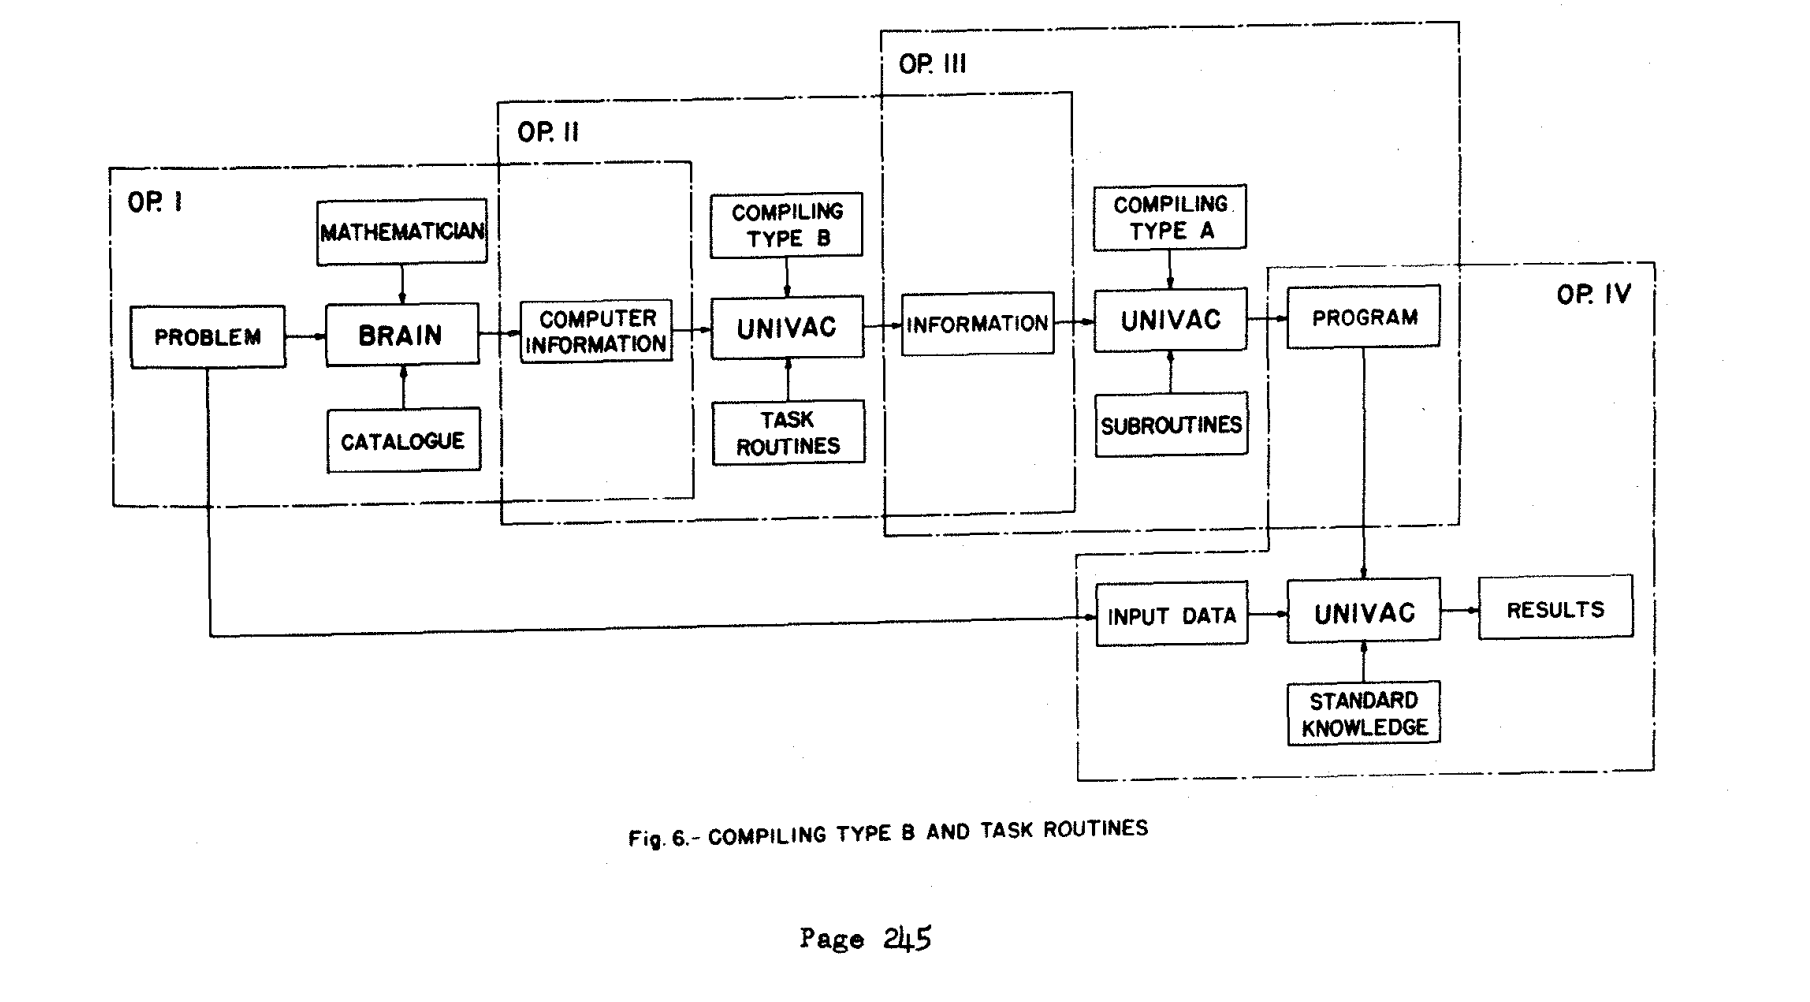
\includegraphics[width=.7\textwidth]{resource/gh_education_of_a_computer_type_fig_6.png}
  \caption{Depiction of \textit{type-B compilation} from Hopper's
  \textit{The Education of a Computer}}
  \label{fig:education-of-a-computer-1952-hopper-f6}
\end{figure}

In this paper, she dubbed her A-0 as a compiler because it was compiling subroutines from a
library into a program, adjusting offsets as necessary. This is far closer to
our modern notion of a linker; its role was to copy machine code from different
locations into a single output program based on an input program \textit{that
was still mostly in machine code}, save for the references to library
subroutines. Her notion of compilation was perhaps closer to the regular
English meaning of compilation, like that of compiling research papers into a
book. Her hope was that "the programmer may return to being a mathematician,"
though her A-0 did not lift the programmer away from machine code to nearly the
same extent as her subsequent efforts would
\cite{education_of_a_computer_1952_hopper}. 
One may also consider this effort
to be the first \textit{standard library}, which would become a major feature
of later compilers and programming languages. This set the stage for compilers
and programming languages providing a default set of useful routines for
programmers to pull from.

The cost of renting a computer remained high relative to the labor cost of
hiring a programmer, thus it was not always economical for computing centers to
use compilers at first. Richard Ridgway and several members of Hopper's team
began testing the A-0 against hand-written programs in the summer of 1952
\cite{ridgway_compiling_routines_1952}. For this study, Richard compared the
computer and labor time spent to calculate a table of values for the equation:

\[
y = e^{-x^2} \sin\left(\frac{x}{2}\right)
\quad \text{for } |x| < 1, \Delta x = 0.01.
\]

After an analysis of the same program written by hand and by the A-0, he
concluded that the A-0 (already considered "antique" by 1952, not more than two years
after Hopper began working on it) was cost-efficient to use for most workloads.
Richard writes in \textit{Compiling Routines}\cite{ridgway_compiling_routines_1952}:

\begin{quotation}
Thus, while more UNIVAC time may be required for the numerical solution of a 
problem as programmed by UNIVAC, more UNIVAC time, \underline{in toto}, is 
consumed by the conventional method. This remains true until the entire problem 
including tis self-contained repetitions is to be repeated, in this case at 
least eighteen times.

If the total preparation time is considered, the problem must be repeated some 
800 times before the conventional programming method overtakes the compiler 
method. In this case, the compiler used was the "antique," or A-0, the first to 
be constructed and the most inefficient.
\end{quotation}

\section{The A-1 and A-2 Compilers}

As Hopper and her team began work on the subsequent A-1 and A-2 compilers,
their motivations shifted away from reducing the tedium of programming to the
economic costs of programming (as is seen in Richard's report).
While computing time was initially far more
costly than human time, as the proportion of computing costs dedicated to human
labor increased over time, the importance of reducing human labor increased as
well.
Her team began working on the A-1 and A-2 in 1953, and the A-2 was
available to UNIVAC customers by the end of the year.
Hopper recruited Herbert Mitchell and Richard Woltman from Aiken's
lab to lead the development of the A-1 and A-2 compilers.
Margaret Harper, Frank Delaney, Mildred Koss, and Richard Ridgway were
the primary developers of these compilers.

There were a number of significant innovations between the A-0 and A-2.
The A-2 performed more of the jobs we associate with compilers today.
Most significantly, by 1954, the A-2 compiler accepted source code
in the form of \textit{pseudocode}, which was a (slightly) more human-friendly
format than plain machine code.
\todo{Some sources reference the A-2 compiler instruction manual,
but I'm unable to find this source online.}
John Backus described the A-2 compiler's 1954 May update as a significant
improvement because of these pseudocode instructions
\cite{hopl_backus_history_of_fortran}.
He placed the A-2 with Laning and Zierler's algebraic compiler and
his own \FTNI{} compiler as the primary compilers of significance in the
mid 1950s.

Along with pseudocode instructions, this compiler also produced
twelve-character error codes to inform the user why something went wrong
during compilation, which must have been tremendously helpful when users
had been accustomed to the alternative.
The compiler worked in two phases, first constructing an index of the
program and then producing the output machine code, informing the user as
it did so.
The a compiler should be friendly to its users was not necessarily a given at
the time; modern compiler tools owe this to Hopper (to the extend that they
are any better than the A-1).

\todo{A-0 and A-1 really had mneumonics for routines that the
compiler new about}.
% \section{The A-1}

\todo{
  the A-2 was a front-end translator to the A-0, more like a complete
toolchain with a front end to a language, a linker and a standard library.}

\section{After the A-2: B-0, FLOW-MATIC, COBOL}

\begin{quotation}
  Pantages: At that point did you have a feeling for what was
  happening, in terms of what you
  were contributing?

  Hopper: No. I've always objected to doing anything over again if I
  had already done it
  once. That was building the compiler. Then I decided there were two
  kinds of people in the
  world who were trying to use these things. One was people who liked
  using symbols -
  mathematicians and people like that. There was another bunch of
  people who were in data
  processing who hated symbols, and wanted words, word-oriented
  people very definitely. And
  that was the reason I thought we needed two languages.
  The data processors did not like symbols, abbreviations that didn't
  convey anything to them.
  They were totally accustomed to writing things in words. So why not
  give them a word-oriented
  language? And that was part of what was behind Flow-Matic B-0,
  which became one of the
  ancestors of COBOL.
\end{quotation}

\todo{later developed the A-3 and AT-3/MATH-MATIC; FLOW-MATIC (B-0,
1956/58), \FTN{}, COBOL}

\begin{quotation}
  B-0, as the business language compiler was designated, became available to
  UNIVAC customers at the start of 1958. Before its completion, Remington Rand
  merged with Sperry Gyroscope Corporation to form Sperry Rand. The marketing
  department of the new company renamed the business language FLOW-MATIC. (In
  addition, AT-3 was renamed MATH-MATIC.) The completed version of
  FLOW-MATIC had
  a rich library of operational verbs that appeared to meet the application
  needs of most businesses.23 These verbs included editing commands so
  information could be formatted before output. Furthermore, FLOW-MATIC provided
  unparalleled flexibility in data designation, thus allowing file names to be
  given complicated descriptions.
\end{quotation}

\begin{quotation}
  her superiors that the proposed business language would only be in English.
  B-0, as the business language compiler was designated, became available to
  UNIVAC customers at the start of 1958. Before its completion, Remington Rand
  merged with Sperry Gyroscope Corporation to form Sperry Rand. The marketing
  department of the new company renamed the business language FLOW-MATIC. (In
  addition, AT-3 was renamed MATH-MATIC.) The completed version of
  FLOW-MATIC had
  a rich library of operational verbs that appeared to meet the application
  needs of most businesses.23 These verbs included editing commands so
  information could be formatted before output. Furthermore,
  FLOW-MATIC provided
  unparalleled flexibility in data designation, thus allowing fi le names to be
  given complicated descriptions.
\end{quotation}

\begin{quotation}
  This was what she originally called the data processing compiler in January,
  1955; it was soon to be known as "B-0," later as the "Procedure
  Translator" [KM 57], and finally as flow-matic [HO 58, TA 60], This language used English
  words, somewhat as math-matic did but more so, and its operations concentrated
  on business applications. The following examples are typical of flow-matic
  operations;
  \cite{history_of_computing_in_the_twentieth_century_1980}
\end{quotation}

\section{Laning and Zierler at MIT}
\label{sec:laning-zierler}

\todo{ Laning and Zierler, 1954. Early 1950s. Inspiration for Backus/\FTN{}.
Worked more like a modern compiler than Hopper's A-0 and A-1.  }

Backus on the Whirlwind\cite{Backus_1980_Programming_in_America_in_1950s}:
\begin{quotation}
  \textbf{5. The Priesthood versus the Laning and Zierler Algebraic Compiler}
  Very early in the 1950s, J. Halcombe Laning, Jr., recognized that
  programming using algebraic expressions would be an important improvement.
  As a result of that insight he and Neal Zierler had the first
  algebraic compiler
  running on WHIRLWIND at MIT in January 1954 [3]. (A private
    communication from the Charles Stark Draper Laboratory indicates
    that they had
  demonstrated algebraic compiling sometime in 1952!) The priesthood
  ignored Laning's insight for a long time. A 1954 article by Charles W. Adams
  and Laning (presented by Adams at the ONR symposium) devotes less than
  3 out of 28 pages to Laning's algebraic system; the rest are devoted to other
  MIT systems. The complete description of the system's method of operation
  as given there is the following
\end{quotation}

\begin{quotation}
  In retrospect, the biggest event of the 1954 symposium on automatic
  programming
  was the announcement of a system that J. Halcombe Laning, Jr. and Niel Zierler
  had recently implemented for the Whirlwind computer at M.I.T.  However, the
  significance of that announcement is not especially evident from the published
  proceedings [NA 524-], 97\% of which are devoted to enthusiastic description s
  of assemblers, interpreters, and 1954-style "compilers".
  \cite{Knuth_TrabbPardo_1976_Early_Development}
\end{quotation}

\begin{figure}[h!]
  \centering
  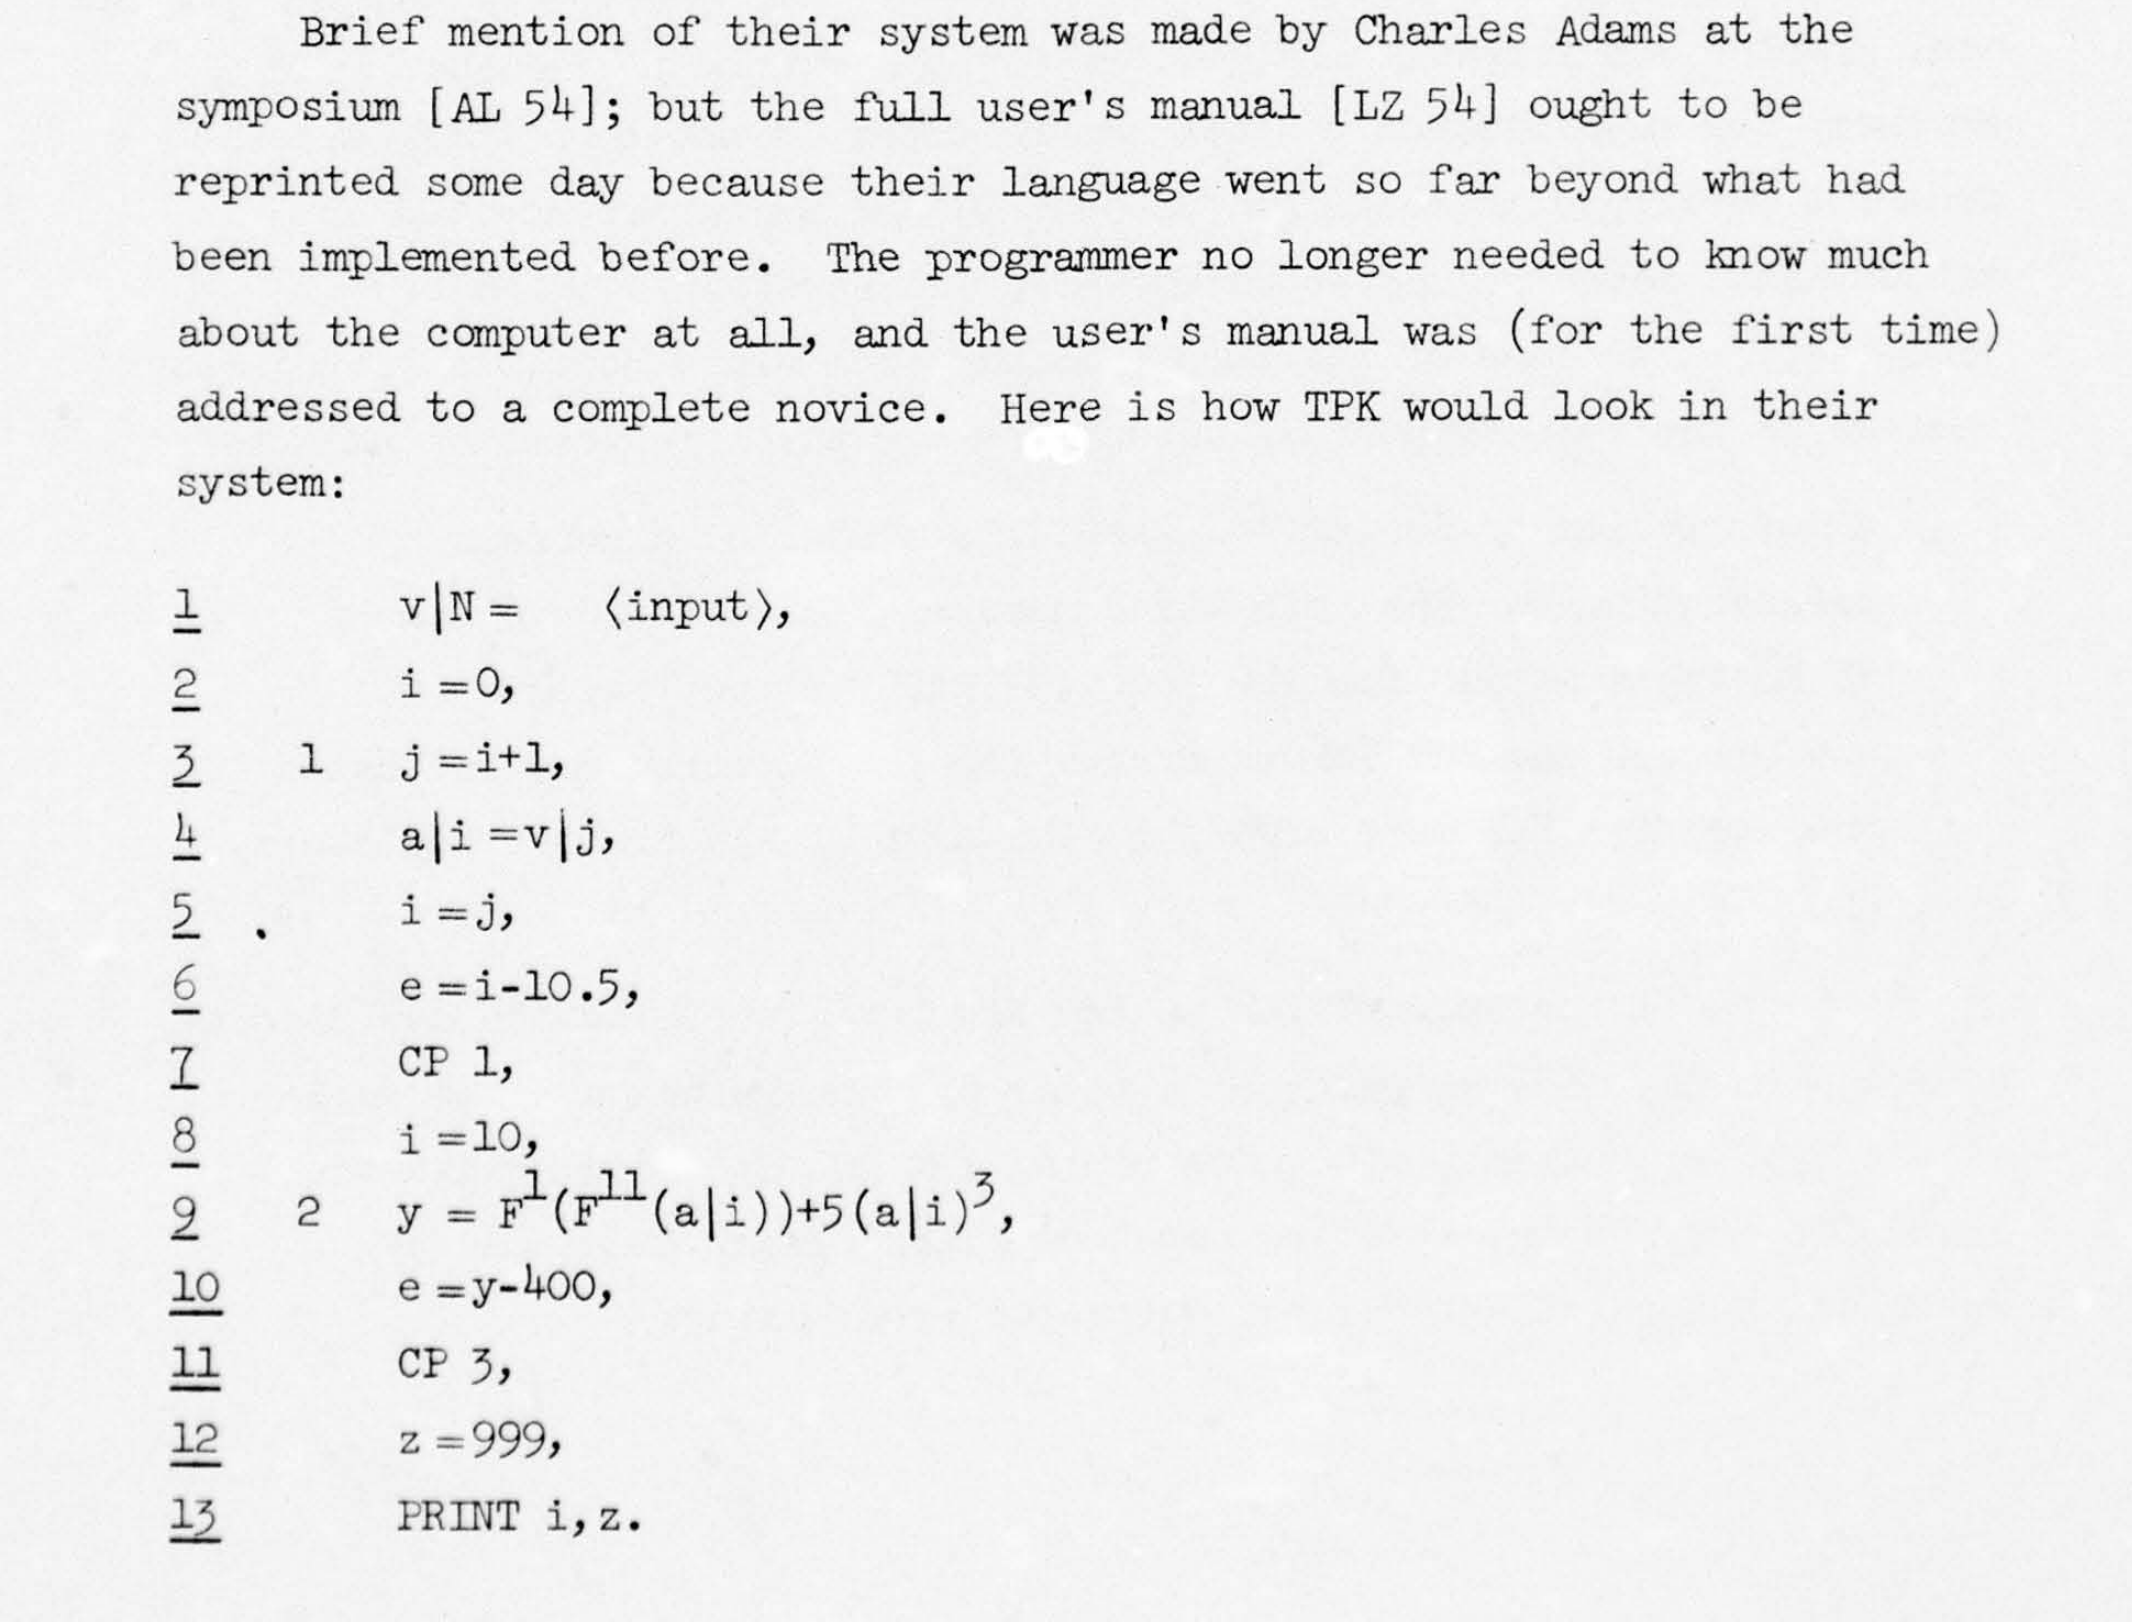
\includegraphics[width=0.5\linewidth]{resource/knuth_pardo_on_laning_zierlers_algebraic_compiler.png}
  \caption{Knuth and Trabb Pardo on Laning and Zierler's Algebraic Compiler}
  \label{fig:knuth-pardo-on-laning-zierler}
\end{figure}

\begin{quotation}
  The first programming system to operate in the sense of a modern compiler was
  developed by J. H. Laning and N. Zierler for the Whirlwind computer at the
  Massachusetts Institute of Technology in the early 1950s. They described their
  system, which never had a name, in an elegant and terse manual entitled "A
  Program for Translation of Mathematical Equations for Whirlwind I,"
  distributed
  by MIT to about one-hundred locations in January 1954.26 It was, in John
  Backus's words, "an elegant concept elegantly realized." Unlike the UNIVAC
  compilers, this system worked much as modern compilers work; that is, it took
  as its input commands entered by a user, and generated as output fresh and
  novel machine code, which not only executed those commands but also kept track
  of storage locations, handled repetitive loops, and did other housekeeping
  chores. Laning and Zierler's "Algebraic System" took commands typed
  in familiar
  algebraic form and translated them into machine codes that Whirlwind could
  execute.27 (There was still some ambiguity as to the terminology: while Laning
    and Zierler used the word "translate" in the title of their manual, in the
  Abstract they call it an "interpretive program.")28
  \cite{new-history-of-modern-computing}
\end{quotation}

\section{John Backus}

IBM did not feel that Aiken and the Harvard Computation Laboratory had given
them sufficient credit for their contributions to the Mark I, which left
Thomas Watson Sr. and the IBM folks bitter about the experience and eager to
produce a new device entirely in-house. This device would become the Selective
Sequence Electronic Calculator, or the SSEC. It was built on 57th Street in
Manhattan, and it was monstrous. Roughly 50 by 100 feet with a giant console
and hundreds of toggle switches and tape units and relays behind glass panels;
there were giant windows that allowed passersby to see the machine in action.

One such passerby was John Backus, a recent Masters graduate from Columbia
University. He was intrigued by the machine, which he mentioned to his tour
guide, who suggested he go upstairs and talk to the boss about it. Robert "Rex"
Seeber gave him a puzzle, which he solved, and he was hired on the spot
\cite{backus_oral_history_2006}.

In 1942, Backus majored in Chemistry at the University of Virginia where he
struggled academically. He was expelled due to poor attendance within the first
year before being drafted into the US Army. He commanded an antiaircraft
battery at Fort Steward, Georgia, remaining in the US for the remainder of
WWII.

While he did not at first find success in academia, he got very good marks on
military aptitude tests. He was directed to the University of Pittsburgh's
engineering program and later to a premedical program at Haverford College near
Philadelphia (which is where he grew up). In 1945 he attended the Flower and
Fifth Avenue Medical School in NYC, but he was still struggling with the
academy. He was uninterested in medicine, feeling that it was all about
memorization. He dropped out after less than a year.

He entered a radio technician school and became interested in math, which led
him to enroll in the math program at Columbia University. The SSEC that would
intrigue him at the IBM computing center was designed at the Watson Scientific
Computing Laboratory at Columbia.

\section{IBM Mathematical FORmula TRANslating System}

At IBM, Backus worked on the SSEC and later the IBM 701 and 704. The main use
of the SSEC was aerospace calculations; programming calculations to predict the
position of the moon was one of the first tasks he was given at IBM. He would
continue writing programs for these machines in spite of their poor usability.
His team's techniques would be used in the lunar missions of the 1960s.

The pain of writing programs for these early machines entirely in machine code
drove him to explore new ways to program. The first of these was a symbolic
notation for floating point arithmetic and address expression calculation
called Speedcoding\cite{backus_oral_history_2006}:

\begin{quotation}
  \textbf{Grady Booch:}
  So then from your experience with the SSEC, you then went on to
  produce Speedcoding, the
  Speedcoder\dots
  What were sort of the things that influenced you to create that in
  the first place?

  \textbf{John Backus:}
  Well, programming in machine code was a pretty lousy business to
  engage in, trying to figure
  out how to do stuff. I mean, all that was available was a sort of a
  very crude assembly program. So I
  figured, well, let's make it a little easier. I mean it was a
  rotten design, if I may say so, but it was better
  than coding in machine language.
\end{quotation}

The IBM 701 did not have an index register, so calculating addresses for array
operations was tedious and error-prone. Speedcoding provided a way to express
these calculations symbolically.

\begin{figure}[h!]
  \centering
  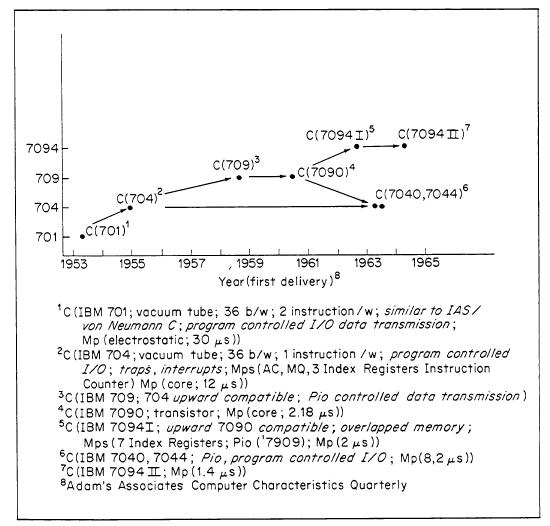
\includegraphics[width=0.5\linewidth]{resource/ibm-7094.jpeg}
  \caption{Excerpt from \textit{The IBM 701--7094 II Sequence: A
    Family by Evolution}
    \cite{Hamming_Feigenbaum_1971_IBM7094}, illustrating the
  instruction structure for summing quantities.}
  \label{fig:ibm7094-example}
\end{figure}

The 704 was the first machine to have such a register; it also had floating
point instructions and core memory, more or less obviating the need for
Speedcoding: "we were moving to the 704, which had built in floating point,
built in index registers, which was all that Speedcoding was supposed to
supply. So what the hell?" \cite{backus_oral_history_2006} He credits himself
with getting index registers and floating point into the 704.

%Here is an example from the IBM Speedcode manual\cite{IBM_1954_Speedcoding}:
%\begin{quotation}
%    Assume that it is necessary to compute the sum of 34 quantities stored in
%    locations 688 through 721 and to store the sum in cell 945.
% Assume further that
%    cell 1013 contains the number zero and that instruction 416 is the next
%    instruction to be executed. The sequence of instructions shown
% below could be
%    used for this purpose:
%
%    \begin{center}
%    \begin{tabular}{cccccccc}
%    \hline
%    LOC & OP$_1$ & R & A & B & C & OP$_2$ & D \\
%    \hline
%    0416 & ADD  & 0 & 1013 & 1013 & 0945 & SETRA & 0000 \\
%    0417 & ADD  & 4 & 0688 & 0945 & 0945 & SKRA  & 0033 \\
%    0418 & NOOP & 0 & 0000 & 0000 & 0000 & TIA   & 0417 \\
%    \hline
%    \end{tabular}
%    \end{center}
%\end{quotation}

\begin{figure}[h!]
  \centering
  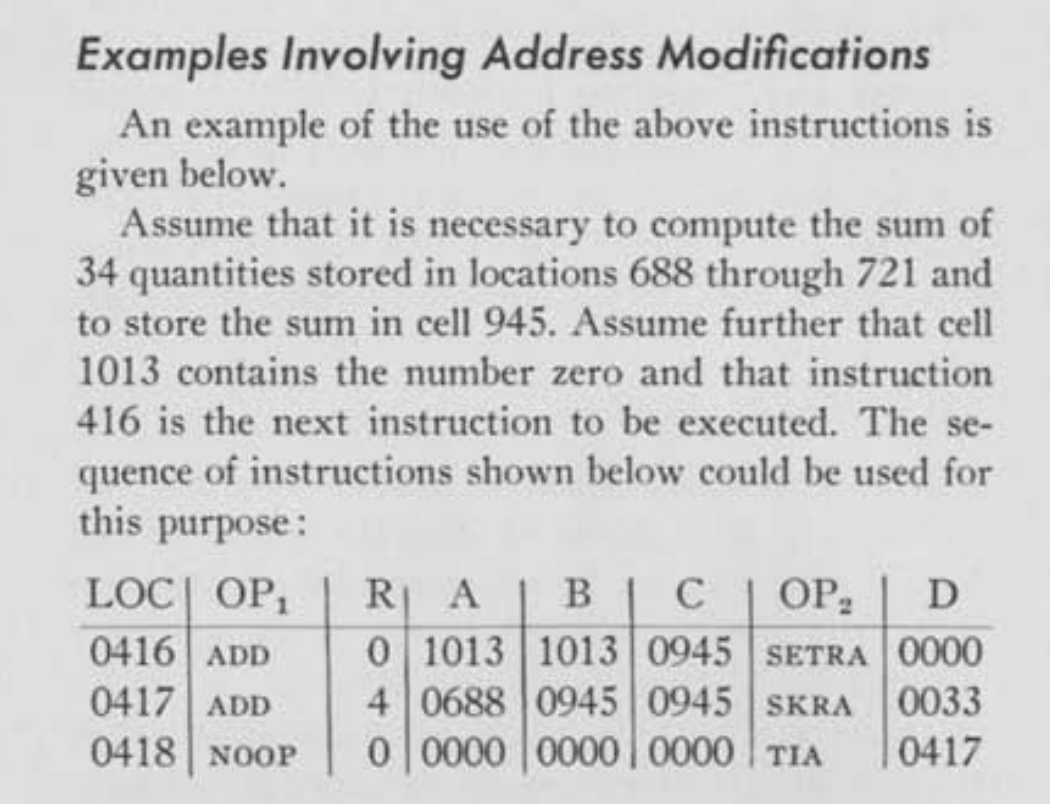
\includegraphics[width=0.5\linewidth]{resource/ibm-speedcoding-example.png}
  \caption{Excerpt from \textit{IBM Speedcoding for the Type 701
    Electronic Data Processing Machine}
  \cite{IBM_1954_Speedcoding}}
  \label{fig:ibm-speedcoding-example}
\end{figure}

Backus did not think all that highly of Speedcoding in retrospect, though it
gained traction in large part due to IBM's marketing power and the number of
users of the 701 relative to the size of the computer market at the time
\cite{Backus_1980_Programming_in_America_in_1950s}. It is unclear whether
Backus's assessment of his own code is accurate or if it's born of humility.

\begin{quotation}
  The success of some programming systems depended on the number of machines
  they would run on. Thus, an elegant system for a one-of-a-kind machine might
  remain obscure while a less-than-elegant one for a production
  computer achieved
  popularity. This point is illustrated by two papers at the 1954 ONR symposium
  One, by David E. Muller, describes a floating point interpretive system for
  the ILLIAC designed by D. J. Wheeler. The other, by Harlan Herrick and myself,
  describes a similar kind of system for the IBM 701 called Speedcoding. Even
  today Wheeler's 1954 design looks spare, elegant, and powerful, whereas the
  design of Speedcoding now appears to be a curious jumble of compromises.
  Nevertheless, Wheeler's elegant system remained relatively obscure (since only
  ILLIAC users could use it) while Speedcoding provided enough conveniences,
  however clumsily, to achieve rather widespread use in many of the eighteen 701
  installations.
\end{quotation}

In 1953, based on his experience with Speedcoding on the 701, Backus proposed
yet another language to elevate the programming experience on the 704. IBM
management supported the proposal. He formed a ten-person team of his own
choosing based out of IBM's Manhattan headquarters, including Irving Ziller,
\todo{list other members}. They released \textit{Preliminary Report,
  Specifications for the IBM Mathematical FORmula TRANslating System,
FORTRAN}\cite{IBM_1954_FORTRAN_Specifications} after about one year of working
together. Roughly two years after its first conception, \FTN{} was released for
the first time. It would go on to ship with every IBM 704 and become the
primary means of programming in the scientific community. Backus could not
stand how slow programming was without a higher-level language, and machines
were expensive; leasing a machine and spending time programming in machine code
wasted money compared to a compiler capable of generating reasonable machine
code (though at the time it usually underperformed hand-written code). Backus
and his team would continue to develop and stabilize this compiler for several
years, though.

\begin{quotation}
  \FTN{} did not really grow out of some brainstorm about the beauty of
  programming in mathematical notation; instead it began with the recognition
  of a basic problem of economics: programming and debugging costs already
  exceeded the cost of running a program, and as computers became faster
  and cheaper this imbalance would become more and more intolerable. This
  prosaic economic insight, plus experience with the drudgery of coding, plus
  an unusually lazy nature led to my continuing interest in making
  programming easier.
  This interest led directly to work on Speedcoding for the 701
  and to efforts to have floating point as well as indexing built into the 704.
  \cite{Backus_1980_Programming_in_America_in_1950s}
\end{quotation}

When Backus was forming his team in January of 1954, he was moved from the Pure
Science department at IBM into the Applied Science department because his boss
Rex Seeber wanted nothing to do with the project. There he found Irving Ziller,
who became his first teammate. By April, they had been joined by Harlan Herrick
who co-authored the Speedcoding paper with Backus at the ONR symposium
\citetitle{Backus_Herrick_1954_Speedcoding} in which they observe:

\begin{quotation}
  The question is, can a machine translate a sufficiently rich mathematical
  language into a sufficiently economical program at a sufficiently low cost to
  make the whole affair feasible?  consider the advantages of being
  able to state
  the calculations\dots for a problem solution in a concise, fairly natural
  mathematical language.
\end{quotation}

The reader should note that it is often incorrectly asserted (at times even by
Backus himself\cite{Backus_1980_Programming_in_America_in_1950s}) that this
came \textit{after} Backus and Ziller had been given a demonstration of Laning
and Zierler's algebraic compiler for the Whirlwind at MIT at the ONR symposium
of 1954. When they received this demonstration, there were already four members
of the \FTN{} team, Irving Ziller, Robert Nelson, Harlan Herrick, and Backus
himself. In Backus's words\cite{Backus_1980_Programming_in_America_in_1950s}:

\begin{quotation}
  The article and the letter therefore show that, much to my surprise, the
  FORTRAN effort was well under way before the ONR symposium and that,
  independently of Laning (but later), we had already formulated more ambitious
  plans for algebraic notation (e.g., Gail bjk) than we were later to find in
  Laning and Zierler's report and see demonstrated at MIT. It is therefore
  unclear what we learned from seeing their pioneering work, despite my mistaken
  assumption over the years that we had gotten our basic ideas from them
\end{quotation}

Indeed, even Grace Hopper at a 1956 symposium made the same assertion:

\begin{quotation}
  A description of Laming and Zierler' s system of algebraic pseudocoding for
  the Whirlwind computer led to the development of Boeing 's BACAIC for the 701,
  FORTRAN for the 704, AT-3 for the Univac, and the Purdue System for the Datotron and. indicated the need for far more effort in the area of algebraic
  translators.
  \cite{Knuth_TrabbPardo_1976_Early_Development}
\end{quotation}

I am not sure who to believe either!

With the support of his new boss Cuthbert Hurd, his family, friends, and his
team, the first report of \FTN{} was released externally to 704 users. This
brought interest from a variety of users, many of whom offered up members of
their teams to help.

\section{\FTN{} Optimization and the First Users}

Setting aside the members of the "priesthood" of computing who were hostile to
the idea of compilers and making programming more accessible, the external
report on \FTN{} brought these contributors into the fold:
\begin{itemize}
  \item Walter Ramshaw at United Aircraft allowed Roy Nutt to work
    with the team; he
    eventually designed and implemented parts of the runtime and I/O features.
  \item Charles W. Adams allowed Sheldon Best to join the team on
    leave from MIT.
  \item Sidney Fernback at the Livermore Radiation Laboratory loaned
    out Bob Hughes.
  \item Harry Cantrell at G.E. was enthusiastic about the project.
\end{itemize}

The team was composed of the following 9 members: David Sayre, Harlan Herrick,
John Backus, Lois Haibt, Robert Nelson, Roy Nutt, Sheldon Best, Richard
Goldberg, and Peter Sheridan.

Most of the skepticism about \FTN{} came from the "priesthood," Backus's
facetious term for the "elite" programmers who thought programming needn't be
made accessible and compilers would never achieve the performance their of
hand-written code. This made the optimization of \FTN{} programs a high
priority for the team; to achieve the widest possible adoption, they would need
to convince even the skeptics that \FTN{} programs could be efficient. In
Backus's 1976 retrospective on programming in the
1950s\cite{Backus_1980_Programming_in_America_in_1950s}, he highlights the
optimization efforts of three members of the original team:

\begin{itemize}
  \item Nelson and Ziller optimized array indexing expressions and
    loop analyses.
    Backus specifies that they could "could move computations from the object
    program to the compiler" which appears to be the first instance of
    constant-folding in a compiler.
  \item Best optimized the use of index registers based on the
    expected hotness of the
    execution path. "As of 1970 there were no known provably optimal
    algorithms for
    the problem he dealt with; his methods were the basis of many subsequent
    storage-allocation algorithms and produced code that is very difficult to
    improve. (For more details of Best's methods see [4, pp. 510-5151.)"
  \end{itemize}

  This is, as far as I can tell, the first concerted effort to produce an
  optimizing compiler.

  \section{Language Specification and Backus-Naur Form}

  \todo{explain BNF and lang specs, tie in with GH algol
  work}\cite{Backus_1980_Programming_in_America_in_1950s}:
  \begin{quotation}
    The notation for syntax description known as BNF offers another example of a
    development which began with a prosaic recognition of a need.
    After involvement
    with two language design efforts-FORTRAN and IAL (ALGOL 58)-it
    became clear, as
    I was trying to describe IAL in 1959, that difficulties were
    occurring due to
    the absence of precise language definitions. In a recent course on
    computability given by Martin Davis, I had been exposed to the work of the
    logician Emil Post and his notion of a "production." As soon as the need for
    precise description was noted, it became obvious that Post's
    productions were
    well suited for that purpose. I hastily adapted them for use in
    describing the
    syntax of IAL. The resulting paper [5] was received with a
    silence that made it
    seem that precise syntax description was an idea whose time had
    not yet come.
    As far as I know that paper had only one reader, Peter Naur. Fortunately, he
    had independently recognized the need for precision; he improved
    the notation
    (replacing oi: by I and := by : =), improved its readability by not
    abbreviating the names of metavariables, and then used it to describe the
    syntax of ALGOL 60 in the definitive paper on that language. He
    thus proved the
    usefulness of the idea in a widely read paper I and it was accepted.
  \end{quotation}
  % \begin{figure}[h!]
  %     \centering
  %     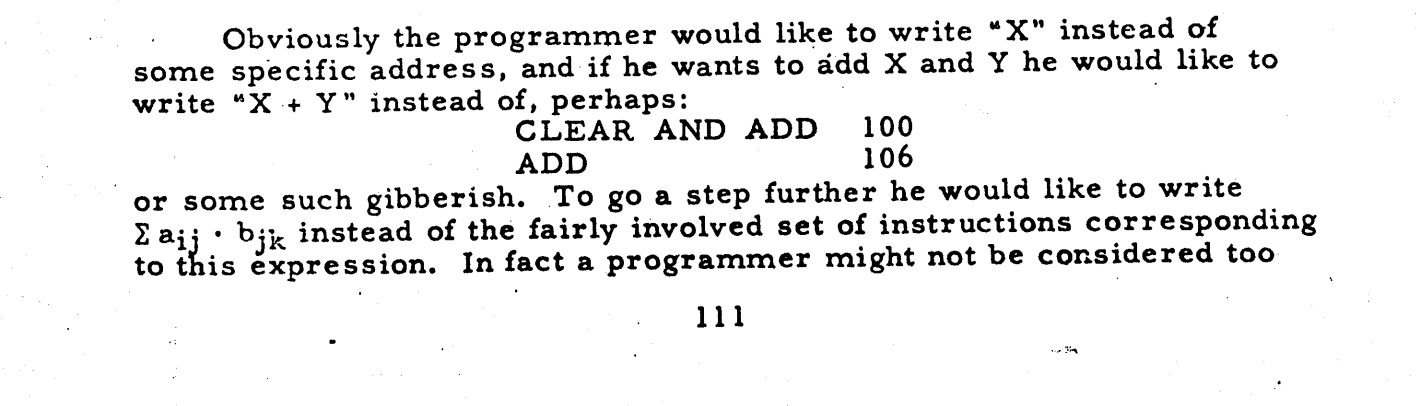
\includegraphics[width=0.5\linewidth]{resource/Backus_Herrick_Speedcoding_ONR_1954.png}
  %     \caption{Excerpt from \citetitle{Backus_Herrick_1954_Speedcoding}}
  %     \label{fig:backus-herrick-speedcoding-onr-1954}
  % \end{figure}

  \todo{Backus wasn't really that involved in fortran II and III and IV.
    The rest of the team took over. He never wrote much fortran and
    doesn't have many thoughts
  about it today other that the "we should be making things higher level."}
  \todo{Backus moved into functional programming. Was never fruitful.
    He became a lab fellow at IBM after Watson Jr started the
    fellowship program,
    so he could kinda play with functional programming and not really
  get much done.}
  \todo{He didn't like Hopper's ideas for COBOL, thought they were
    crazy and too complex.
    Didn't like algol either. Really just wanted to make things
    simpler and higher level
  and easier to use. Pushed back against the priesthood.}
  \todo{the priesthood didn't like fortran because it made things easy.
    Backus resisted this urge at every point in his career.
    Like GH, he wanted programming to be easy and accessible
  (tho he didn't like her direction)}

  \begin{quotation}
    Though the FORTRAN operator's manual was completed by the fall of 1956, the
    compiler itself was not distributed to IBM 704 installations
    until April 1957.
    Within a year after distribution, half of the IBM 704
    installations were using
    FORTRAN to solve more than half of all mathematical prob-lems.16
    Subsequently,
    compilers were produced for the IBM 705 and the IBM 650, quickly
    making FORTRAN
    the most widely used automatic program of its day. By 1961, UNIVAC users
    demanded a compatible FORTRAN compiler and abandoned Hopper's MATH-MATIC.
    \cite{grace_hopper_and_the_invention_of_the_information_age_2009}
  \end{quotation}

  \begin{quotation}
    It describes the system which will be made available during late
    1956, and is
    intended to permit planning and fortran coding in advance of that
    time [p. 1],
    Object programs produced by fortran will be nearly as efficient as those
    written by good programmers [p. 2], "Late 1956" was, of course, a
    euphemism for
    April 1957. Here is how Saul Rosen described fortran's debut [RO
    64, p. 4]: Like
    most of the early hardware and software systems, fortran was late
    in delivery,
    and didn't really work when it was delivered.
    \cite{history_of_computing_in_the_twentieth_century_1980}
  \end{quotation}

  \begin{quotation}
    It is not my intention to give a complete description of either; hence this
    section will describe only the main highlights of FORTRAN development. The
    earliest significant document that seems to exist 1s one marked
    "PRELIMINARY REPORT, Specifications for the IBM Mathematical FORmula
    TRANslating System, FORTRAN", dated November 10, 1954 and issued by the
    Programming Research Group, Applied Science Division, of IBM.
    \cite{sammet_programming_languages_history_and_fundamentals_1969}
  \end{quotation}

  \begin{quotation}
    Laning and Zierler's algebraic compiler served as evidence that prestigious
    institutions such as MIT were taking automatic programming
    seriously, prompting
    Backus to write Laning a letter shortly after the May symposium.
    In the letter,
    Backus informed Laning that his team at IBM was working on a
    similar compiler,
    but that they had not yet done any programming or even any
    detailed planning.12
    To help formulate the specifications for their proposed language, Backus
    requested a demonstration of the algebraic compiler, which he and Ziller
    received in the summer of 1954. Much to their dismay, the two
    experienced firsthand the efficiency dilemma of compiler-based
    language design. The MIT
    source code was commendable, but the compiler slowed down the Whirlwind
    computer by a factor of 10. Since computer time was so dear a
    commodity, Backus
    realized that only a compiler that maximized efficiency could
    hope to compete
    with human programmers. Despite this initial disappointment, Laning and
    Zierler's work inspired Backus to attempt to build a compiler that could
    translate a rich mathematical language into a sufficiently
    economical program
    at a relatively low cost.13
    \cite{grace_hopper_and_the_invention_of_the_information_age_2009}
  \end{quotation}

  \pagebreak
  \section{Timeline}
  \pagebreak
\begin{figure}[h]
\begin{luacode}
timeline.draw_timeline({ 
    start_year = 1942,
    end_year = 1957,
    marker_interval = 1,
    show_year = false,
    events = {
        {1942, "Zuse conceptualizes first high-level language \\textit{Plankalkül}"},
        {1944, "Automatic Sequence Control Calculator started working"},
        {1950, "Rutishauser ran the Z4 as a compiler at ETH", position=1950},
        {1951, "B{\"o}hm develops practical compiler for PhD thesis at ETH"},
        {1951.5, "Hopper begins work on the A-0 compiler for the UNIVAC I"},
        {1952, "Hopper presents \\textit{Automatic Programming} at ACM"},
        -- {1952.5, "Alick Glennie develops first compiler in the modern sense for the U of Manchester Mark I"},
        {1952.5, "Alick Glennie develops compiler for Mark I "},
        {1953, "Hopper's team completes the A-1"},
        {1953.3, "Hopper's team completes the A-2"},
        {1953.6, "Hopper gives presentation to UNIVAC users on the A-2"},
        {1953.9, "Numerous US government agencies have adopted the A-2"},
        {1954.5, "John Backous at IBM begins work on \\ftn{}"},
        {1954.9, "Nora Moser of US Army sends Hopper modifications to the A-2"},
        {1957, "John Backous at IBM released the first \\ftn{} compiler, the first commerical compiler"},
    },
})
\end{luacode}
\caption{Early compiler history, 1940--1960}
\label{fig:dawn-timeline}
\end{figure}



\chapter{Software, 1960-1980ish}
\todo{shit got crazy; became important, needs more focus/attention.}
\section{The Software Crisis}
\begin{quotation}
    Despite great strides in software, programming always seemed to be in a state of crisis and 
always seemed to play catch-up to the advances in hardware. This crisis came to a head in 1968, just 
as the integrated circuit and disk storage were making their impact on hardware systems. That year, 
the crisis was explicitly acknowledged in the academic and trade literature and was the subject of a 
NATO-sponsored conference that called further attention to it.Some of the solutions proposed were a 
new discipline of software engineering,more formal techniques of structured programming, and new 
programming languages that would replace the venerable but obsolete COBOL and FORTRAN. Although 
not made in response to this crisis, the decision by IBM to sell its software and services separately 
from its hardware probably did even more to address the problem. It led to a commercial software 
industry that needed to produce reliable software in order to survive. The crisis remained, however, 
and became a permanent aspect of computing. Software came of age in 1968; the following decades would 
see further changes and further adaptations to hardware advances.
\cite{history_of_modern_computing_2003_ceruzzi}
\end{quotation}
\todo{DEC PDP-8 and PDP-11; IBM System/360 and OS/360; Multics; Unix; C}As the 1960s progressed, 
the notion of 
\textit{software} became more established,and the programs being written served the authors to a 
much greater extent.Prior to the 1960s, programs were often tailor-made for a specific 
machine.There was no hope of re-using the program on another machine.For most of the users, their 
organization had spent a considerable portion of their budget on their system, and they were 
expected to use it for a long time. Retargetable compilers did not exist.Michael Mahoney made a 
strong statement to this end rather early on 
\cite[The Structures of Computation]{the-first-computers-2002}:
\begin{quotation}
    The kinds of computers we have designed since 1945 and the kinds of programs we have written for 
them reflect not the nature of the computer but the purposes and aspirations of the groups of people 
who made those designs and wrote those programs, and the product of their work reflects not the 
history of the computer but the histories of those groups, even as the computer in many 
cases fundamentally redirected the course of those histories.
\end{quotation}
\todo{1945 was too early for this strong of a statement;how can one argue that software reflected 
the authors when it was so dependent on the hardware?
They were still very dependent on the specific machine they were working on and
could not solely focus on their own problems.}
\section{Seymore Cray}
\begin{quotation}
    The CDC 160 and the Origins of the MinicomputerThe Whirlwind (a computer prototype built at 
MIT) had a word length of only 16 bits, but the story of commercial minicomputers really begins with 
an inventor associated with very large computers: Seymour Cray. While at UNIVAC Cray worked on the 
Navy Tactical Data System (NTDS), a computer designed for navy ships and one of the first 
transistorized machines produced in quantity. Around 1960 Control Data, the company founded in 1957 
that Cray joined, introduced its model 1604, a large computer intended for scientific customers. 
Shortly thereafter CDC introduced the 160, designed
\cite{nothing_new_since_von_neumann_2000}
\end{quotation}
\section{The DEC VAX and the IBM System/360}
\begin{quotation}
    Through the 1980s the dominant mainframe architecture continues to be a descendent of the IBM 
System/360, while the dominant mini was the DEC VAX, which evolved as a 32 bit extension of the 
16-bit PDP-11.
\cite{nothing_new_since_von_neumann_2000}
\end{quotation}
\section{Aho Before Bell Labs}
\section{Aho, Ullman, and Bell Labs}
\todo{Software (and compilers!) starts to become a real discipline!Ullman was older and further 
along than Aho, and Hopcraft came to Princeton and became Aho's advisor.}
\begin{quotation}
    One of the first people that I met at Princeton was a Columbia graduate by thename of Jeffrey 
Ullman. He had just gotten his undergraduate degree fromColumbia University and also had come to 
study digital systems in the EEdepartment at Princeton. So, he and I became close friends. When we 
graduatedfrom Princeton, we both joined the newly formed Computing Sciences ResearchCenter at Bell 
Labs. There we developed a lifelong collaboration on subjectsranging from algorithms, programming 
languages, to the very foundations ofcomputer science. I was very fortunate to have met some of the 
greatest peoplein the field and to have gotten to know them and work with them. You learn somuch by 
working with the best people in the field. So, I felt very blessed because I had this kind of 
background
\dots
Hsu: Before we jump into Bell Labs more deeply, could you maybe explain-- talk about your PhD 
thesis,but try to explain it to somebody who, maybe like a museum goer who doesn't really know much 
about computer science and linguistics.

Aho: This is interesting. As I mentioned, Hopcroft told me, "Find your own research problem." He 
did teach a course in automata and language theory, so I got introduced to formal language theory 
and automata theory, at least, as it was known at that time. I was interested in programming 
languages and compilers. What I noticed was that a programming language has a syntax and a 
semantics. All languages have a syntax and a semantics. If you want to write a translator for a 
programming language, or even a natural language, you have to understand the syntax and semantics of 
your source language and the target language
\dots
Hansen: 1967, and you followed Ullman there. He had already joined Bell Labs before.

Aho: A few months before me.

Hansen: A few months before. And what group was it that you joined?

Aho: I was interviewed by a department head by the name of Doug McIlroy. He was an 
applied mathematician from MIT. He had been at Bell Labs for a few years before me. Amongst other 
things, he had co invented macros for programming languages and he's also in this class of one of the 
smartest people I've ever met.Jeff wanted to go to academia a little bit earlier than I did, like 
many years earlier. He stayed at Bell Labs for a few years and went to PrincetonUniversity where he 
joined the faculty of the electrical engineering department, but he would come and spend one day a 
week consulting at Bell Labs.His consulting stint was he would come Fridays and sit in my office 
all day.The conversations that we'd have would range over all sorts of topics, and sometimes he'd 
mentioned that he was working on a problem with a colleague atPrinceton, and after describing the 
problem, I might say, "You're kidding," and he said, "Oh, you're right. The solution is obvious, 
isn't it?" I don't know whether I would say dynamic programming or whatever, but several papers 
came out of this intense collaboration, and we got to the point where we could communicate with just 
a few words. We had a very large, shared symbol table.
\cite{aho_oral_history_2022}
\end{quotation}
\begin{quotation}
    But as Unix was being developed, Ken Thompson created the first two versions ofUnix using 
assembly language. He had joined Bell Labs at roughly the same time I had. He was there maybe six 
months or so ahead of us, and he had been assigned to work on the Multics project that BellLabs was 
part of with MIT and GE. When Bell Labs got tired of pouring money into Multics and not getting the 
operating system that it had wanted, it abandoned the project and left Ken Thompson to his 
own devices. Ken thought there were some good ideas in Multics. Being the genius that he was, he 
said, I can do it much more simply and much more elegantly. So he created a rudimentary version of 
Unix and thenkept writing and polishing it. Dennis Ritchie came on the scene. Ken had also created 
a programming language, B. The B was maybe the first letter of BCPL. Who knows? But when Dennis 
Ritchie looked at it, he said, what B needs is a decent type system. So he put a decent type system 
on B, and created theC programming language. Thompson and Ritchie wrote the third version of Unix 
using the newly createdC programming language. I became an early adopter of C, and I had C wired in 
my fingertips, so I could write C programs quite readily, and of course, there were all these neat 
tools that accompanied the programming environment on Unix. There were the text editors. I don't 
know whether you've ever heard of the ED editor or the QED editor that was at MIT as part of 
Multics. QED had regular expressions in it. This triggered my interest in regular expressions. Ken 
Thompson had written a program called grep for doing pattern matching on text files, and it had a 
very limited form of regular expressions when I encountered it.
\cite{aho_oral_history_2022}
\end{quotation}
\begin{quotation}
\textbf{Collaboration with Ullman}

Aho is best known for the textbooks he wrote with Ullman, his co-awardee. 
The two were full time colleagues for three years at Bell Labs, but after 
going back to Princeton as a faculty member Ullman continued to work one day a 
week for Bell.They retained an interest in the intersection of automata theory 
with formal language. In an early paper, Aho and Ullman showed how it was 
possible to makeKnuth's LR(k) parsing algorithm work with simple grammars that 
technically did not meet the requirements of an LR(k) grammar. This technique 
was vital to theUnix software tools developed by Aho and his colleagues at Bell 
Labs. That was just one of many contributions Aho and Ullman made to formal 
language theory and to the invention of efficient algorithms for lexical 
analysis, syntax analysis, code generation, and code optimization. They 
developed efficient algorithms for data-flow analysis that exploited the 
structure of "gotoless" programs, which were at the time just becoming the norm.
\cite{aho_turing_award_2020}
\end{quotation}
\begin{quotation}
\textbf{The Early History of Software, 1952-1968 101}

In the early 1960s computer science struggled to define itself and its 
purpose,in relation not only to established disciplines of electrical 
engineering and applied mathematics, but also in relation to—and as something 
distinct from—the use of computers on campus to do accounting, record keeping, 
and administrative work.58 Among those responsible for the discipline that 
emerged, Professor George Forsythe of Stanford's mathematics faculty was 
probably the most influential. With his prodding, a Division of Computer Science 
opened in the mathematics department in 1961; in 1965 Stanford established a 
separate department, one of the first in the country and still one of the 
most well-regarded.59
\cite{history_of_modern_computing_2003_ceruzzi}
\end{quotation}
\todo{Dragon book; all the books Aho, Ullman and others worked on together.}
\section{Compiler-Compilers}
\todo{Yacc and Lex made with Aho's help. then everyone started making mini languages.AWK. 
"Kernighan and Cherry developed a little language for specifyingmathematics called EQN using these 
tools"}
\begin{quotation}
    People started using the Kernighan and Lorinda Cherry EQN tool to specify mathematics in their 
documents and in the research papers that they were writing. They would feed the EQN specification 
into the typesetting program roff
\dots
Knuth adopted the EQN language to include in the TeX typesetting system, and in LaTeX. It's 
basically Kernighan and Cherry's way of specifying mathematics. These software tools had a great 
deal of influence, and Kernighan and Cherry enjoyed the fruits of parsing theory and formal language 
theory in using the tools Lex and Yacc to create their EQN typesetting language. Knuth has this 
saying that the best theory is motivated by practice and the best practice by theory. I internalized 
that with my early experience in the Computing SciencesResearch Center because I found that the 
theory that we were developing in computer science could be applied to document preparation systems, 
programming languages, compilers, and so on. It was really avery productive environment. I taught 
courses on compiler design at local universities, and then when I went to Columbia, I would teach 
the course on programming languages and their translators
\dots
I might point out that the first Fortran compiler developed by IBM in the 1950s took 18 staff years 
to create. In my programming languages and compilers course, I organized the students into teams of 
four or five. Each team had to create their own programming language, and then write a translator 
for it, and in all the time that I taught the course for almost 25 years at Columbia to thousands of 
students, never did a team failed to deliver a working compiler in the 15-week course, and I 
attribute that to the abstractions
\cite{aho_oral_history_2022}
\end{quotation}
\begin{quotation}
    Aho: Okay. AWK is a programming language that was created by me, Brian 
Kernighan, and Peter Weinberger.

Hsu: And it's your three initials that are in.

Aho: Yes. I'm the A in AWK. Weinberger is the W in AWK and Kernighan is the 
K in AWK.We thought that it was just a throwaway tool for us, nobody really 
would be interested in it. But it's amazing how much routine data processing 
there is in the world.The reason the language got to be known as AWK was because 
when our colleagues would see the three of us in one office or another, and when 
they'd walk past the open door, they'd say, AWK, AWK, AWK as they were going 
down the corridor. So we had no choice but to call it AWK because of the 
good-natured ribbing we got from our colleagues, and because at some Unix 
conference, they passed out t-shirts that had AWK,and the error message saying 
"bailing out on or near line five" on them.
\end{quotation}
\todo{Ratfor, AMPL, other Kernighan languages.}
\todo{continue with typesetting...}
\section{The Dragon Book}
\begin{quotation}
    Jeff had bought into this idea that it's good for your career to write a 
book about what you're working on. In the '70s, with all this work on Unix and 
C, there was a lot of interest in creating new programming languages and 
compilers. As with the algorithms book, what we did was we performed research 
on efficient algorithms for parsing and for some of the other phases of 
compilation, wrote papers on those  and presented them at conferences. But we 
took the important ideas that we developed and the community had developed over 
several decades and codified them into what are now called the dragon books. The 
first dragon book was published in 1977.We did have theorems and proofs in the 
book, and Jeff had this brilliant idea that the book should have a cover with a 
fierce dragon on it representing the complexity of compiler design,and then a 
knight in armor with a lance. The armor and the lance were emblazoned with 
techniques from formal language theory and compiler theory to slay the 
complexity of compiler design
\dots
In the 1980s, more was known about how to construct efficient compilers. We 
invited Ravi Sethi as a third coauthor, he was at Bell Labs at the time, to join 
us in creating the second version of the dragon book. In the first version, the 
dragon was in red. This second version, the dragon was-- sorry. In the first 
version it was in green. In the second version the dragon was in red. What was 
interesting about the red dragon book was there was a movie that was created in 
1995 titled Hackers with a young Angelina Jolie in it, and in the movie, there 
is the uber hacker that's explaining to the new hackers what you have to read to 
become an uber hacker. He shows them 10 papers and books that you must read, and 
one of them was the red dragon book. When my two children saw this movie, and 
they had seen the red dragon book at home, this is the first time they thought 
their old man was really something because he had one of his books in a 
Hollywood movie. It shows what you have to do to impress your kids these days. 
The red dragon book was 800 pages. In2007, we invited Monica Lam as a fourth 
coauthor to create a third version of the dragon book that had a purple dragon 
on the cover and it was close to a thousand pages. None of us had the heart to 
write a fourth book at this point because it just shows how much new knowledge 
had been created in the area of programming languages and compilers and their 
translators, and we continued to do research in this area to keep up with it.
\cite{aho_oral_history_2022}
\end{quotation}
\todo{Bjarne Stroustrup, C++ (1979); Dennis Ritchie, C (1972); Ken Thompson, B (1969); Brian 
Kernighan, AWK (1977), AMPL (1976), co-author of The C Programming Language (1978)}
\section{Commodification}
\todo{Bill Gates and Paul Allen (Microsoft) | Microsoft BASIC (1975) | 
Developed the first critical piece of commercial software for personal 
computers,establishing the doctrine that software should be a purchased, 
proprietarycommodity. Sun microsystems, each part of the company needed to sell 
to all the others,reason why their compiler was paid; proprietary Unix;}
\pagebreak
\section{Timeline}
\begin{figure}[h]
\begin{luacode}
    local start = 1965
    local _end = 1980
    timeline.draw_timeline({    
        start_year = start,    
        end_year = _end,    
        marker_interval = 5,    
        show_year = false,    
        line_always = true,    
        events = {        
        {1967, "Aho joins Bell Labs shortly after Ullman"},        
        {1972, "C"},        
        {1977, "Brian Kernighan, AWK",delta=-.5},        
        {1977, "The Dragon Book first published",delta=.5},        
        {1979, "Bjarne, C++"},    },})
tex.sprint(string.format("\\caption{TBD, %d--%d}", start, _end))
\end{luacode}
\label{fig:tbd-timeline}
\end{figure}



\chapter{Uniformity, 1970-1980}
\chapter{Freedom, 1980-1990}
\chapter{Dotcom, 1990-2000}
\chapter{Codesign, 2010-Present}

\chapterstar{Quotes}

This section should not be included in the final copy;
it contains quotes and bibliographic references that may be useful in the writing of the book.

\vspace{1em}

\quotesection{allen_catalogue_1971}

One of the earliest publications about compiler optimizations. Mentions inlining/IPO.

\begin{quotation}
The term \textit{optimization} is a misnomer in that it is not generally clear that a particular, so called, optimizing transformation even results in an improvement to the program. A more correct term would be "amelioration."
\end{quotation}

\quotesection{the_first_computers_2002}

\begin{quotation}
The chief programmer of Mark I, Richard M. Bloch, kept a notebook in which he wrote out pieces of code
that had been checked out and were known to be correct. One of Bloch's routines computed sines for
positive angles less that 45 degrees to only ten digits. Rather than use the slow sine unit built into the
machine, Grace Hopper simply copied Dick's routine into her own program whenever she knew it would suit
her requirements. This practice ultimately allowed the programmers to dispense with the sine, logarithm, and
exponential units altogether. Both Bloch and Bob Campbell had notebooks full of such pieces of code. Years
later, the programmers realized that they were pioneering the art of subroutines and actually developing the
possibility of building compilers.
\end{quotation}

\begin{quotation}
There were sets of instructions for integers, floating-point numbers, packed decimal numbers, and character
strings; operating in a variety of modes. This philosophy had evolved in an environment dominated by
magnetic core memory, to which access was slow relative to processor operations. Thus it made sense to
specify in great detail what one wanted to do with a piece of data before going off to memory to get it. The
instruction sets also reflected the state of compiler technology. If the processor could perform a lot of
arithmetic on data with only one instruction, then the compiler would have that much less work to do. A rich
instruction set would reduce the "semantic gap" between the English-like commands of a high-level
programming language and the primitive and tedious commands of machine code. Cheap read-only memory
chips meant that the designer could create these rich instruction sets at low cost if the computer was microprogrammed.
\end{quotation}

p. 270
\begin{quotation}
In the following sections, expressions such as "hardware", "software", "machine language", "compiler",
"architecture" and the like are used freely, although they were unknown in 1950. They only arrived a decade
later, but the underlying concepts were quite familiar to us.
\end{quotation}

\begin{quotation}
    We also made some hardware changes. Rutishauser, who was exceptionally creative, devised a way of
letting the Z4 run as a compiler, a mode of operation which Zuse had never intended. For this purpose, the
necessary instructions were interpreted as numbers and stored in the memory. Then, a compiler program
calculated the program and punched it out on a tape. All this required certain hardware changes. Rutishauser
compiled a program with as many as 4000 instructions. Zuse was quite impressed when we showed him this
achievement.
\end{quotation}

\quotesection{grace_hopper_and_the_invention_of_the_information_age_2009}

\begin{quotation}
Though it is sometimes difficult to identify the motivation behind particular i
nventions, it appears that a dearth of talented programmers, a personal frustrat
ion with the monotony of existing programming techniques, and the lack of resour
ces made available by senior management at Remington Rand to support computer cl
ients led Hopper to invent the technologies and techniques, such as the compiler
, that allowed the computers to, in effect, help program themselves. Interesting
ly enough, as her A-0 compiler evolved into the A-1 and the A-2, Hopper’s reason
ing in regard to the invention changed. Compilers became less about relieving pr
ogrammers of the monotony of coding and more about reducing programming costs an
d processing time.
\end{quotation}

\textit{Programming} was considered the action of writing machine code directly;
writing code in a high-level language was not even considered programming.
The motivation for writing Hopper's first compiler was to offload this task
to the computer itself.

\begin{quotation}
First and
foremost, the central motivations for automatic programming
were far more personal in the 1952 paper. With the construction
of a functioning compiler, Hopper hoped, "the programmer
may return to being a mathematician." Though Hopper had
sincerely enjoyed the challenge of coding since first being introduced to computers 8 years earlier, she wrote, "the novelty of
inventing programs wears off and degenerates into the dull labor
of writing and checking programs. The duty now looms as an
imposition on the human brain." By teaching computers to
program themselves, Hopper would be free to explore other
intellectual pursuits 
\end{quotation}

\begin{quotation}
These computing pioneers, according to
Hopper, created machines and methods that removed the arithmetical chore from the mathematician. This chore, however, was
replaced by the new burden of writing code, thus turning mathematicians into programmers. Hopper's paper boldly offers the
next step in the history of computing: shifting the humanmachine interface once again so as to free the mathematician
from this new burden, and making "the compiling routine be
the programmer and perform all those services necessary to the
production of a fi nished program."
\end{quotation}

\begin{quotation}
He [the mathematician] is supplied with a catalogue of subroutines. No
longer does he need to have available formulas or tables of elementary
functions. He does not even need to know the particular instruction
code used by the computer. He needs only to be able to use the catalogue to supply information to the computer about his problem.20
The “catalogue of subroutines” was a menu that listed all the
input information needed by the compiler to look up subroutines in the library, assemble them in the proper order, manage
address assignments, allocate memory, transcribe code, and create
a fi nal program in the computer’s specifi c machine code.21 A
subroutine entry in the catalogue consisted of a subroutine
“call-number” and the order in which arguments, controls, and
results were to be stated. The call-number identifi ed the type of
subroutine (t for trigonometric, x for exponential, etc.), specified
transfer of control (entrance and exit points in each subroutine),
and set operating and memory requirements. In fact, language
such as “call-number” and “library” compelled Hopper to name
her program generator a “compiler,” for it compiled subroutines
into a program in much the same way that historians compile
books into an organized bibliography.22
\end{quotation}

\begin{quotation}
A program generated by a compiler could not only be
run as a stand alone program whenever desired; it also “may itself
be placed in the library as a more advanced subroutine.” This
suggested that subroutine libraries could increase in size and
complexity at an exponential rate, thus enabling mathematicians
to solve problems once deemed impossible or impractical.23
\end{quotation}

\begin{quotation}
Hopper ends the paper by establishing a short-term roadmap
for the future development of compilers. She describes a “typeB” compiler, which, by means of multiple passes, could supplement computer information provided by the programmer with
self-generated information. Such a compiler, she imagines, would
be able to automate the process of solving complex differential
equations. To obtain a program to compute $f(x)$ and its first $n$
derivatives, only $f(x)$ and the value of n would have to be given.
The formulas for the derivatives of $f(x)$ would be derived by
repeated application of the type-B compiler.24
Hopper also admits that the current version of her compiler
did not have the ability to produce efficient code. For example,
if both sine and cosine were called for in a routine, a smart
programmer would fi gure out how to have the program compute them simultaneously. Hopper’s compiler would embed both
a sine subroutine and a cosine subroutine in sequence, thus
wasting valuable memory and processing time. Hopper states
boldly that the skills of an experienced programmer could eventually be distilled and made available to the compiler. She concludes as follows:
\end{quotation}

\begin{quotation}
Although the test results appear to be a smashing endorsement
of the A-0 compiler, Ridgway dedicates a substantial amount of
his paper to the ineffi ciency of run-programs. (A “run-program”
was the fi nal product of the compiler process. Today, such a
program is called object or machine code.) During the 5 months
since Hopper had introduced compilers, critics had pointed out
that run-programs generated by compilers were less effi cient than
those created by seasoned programmers... 

Furthermore, an hour of computer time was far more costly in 1952 than an hour of programmer time. 
\end{quotation}

\begin{quotation}
Ridgway acknowledged that using compilers took up more
computer time, both as a result of compiling a program and as
a consequence of ineffi cient code. But “in this case,” he argued,
“the compiler used was the ‘antique,’ or A-0, the fi rst to be
constructed and the most ineffi cient.” Ridgway was confi dent
that Hopper and her team at the Computation Analysis Laboratory would construct new compilers that “squeezed” coding
into “neat, effi cient, and compact little packages of potential
computation.”29
\end{quotation}

\quotesection{hopl_keynote}
\begin{quotation}
    Mark I had built-in programs for sine, cosine, exponential, arctangent, .-... On the
other hand, because they were wired into the machine, they had to be completely general.
Any problem that we solved, we found we did not need complete generality; we always
knew something about what we were doing--that was what the problem was. And the answer was--we started writing subroutines, only we thought they were pieces of coding.
And if I needed a sine subroutine, angle less than zr/4, I'd whistle at Dick and say, "Can I
have your sine subroutine?" and I'd copy it out of his notebook. We soon found that we
needed just a generalized format of these if we were going to copy them, and I found a
generalized subroutine for Mark I. With substitution of certain numbers, it can be copied
into any given program. So as early as 1944 we started putting together things which would
make it easier to write more accurate programs and get them written faster. I think we've
forgotten to some extent how early that started.
\end{quotation}


\nocite{*}
\printbibliography[heading=bibintoc]
\end{document}
